%% Hashmon Overleaf-ready paper
\documentclass[sigconf]{acmart}

\AtBeginDocument{%
  \providecommand\BibTeX{{%
    Bib\TeX}}}

\copyrightyear{2026}
\acmYear{2026}
\setcopyright{none}
\acmConference[FTE4312]{FTE4312 Course Project}{April 2026}{Shenzhen, China}
\acmBooktitle{FTE4312 Course Project Report}
\settopmatter{printacmref=false}
\renewcommand\footnotetextcopyrightpermission[1]{}

\usepackage{booktabs}
\usepackage{subcaption}
\usepackage{enumitem}
\usepackage{graphicx}
\usepackage{microtype}
\usepackage{array}
\usepackage{float}
\usepackage{dblfloatfix}

\graphicspath{{./}{graphs/}}
\setkeys{Gin}{width=\linewidth,height=0.25\textheight,keepaspectratio}
\setlength{\textfloatsep}{12pt plus 2pt minus 2pt}
\setlength{\floatsep}{10pt plus 2pt minus 2pt}
\setlength{\intextsep}{10pt plus 2pt minus 2pt}
\renewcommand{\topfraction}{0.9}
\renewcommand{\bottomfraction}{0.85}
\renewcommand{\textfraction}{0.08}
\renewcommand{\floatpagefraction}{0.8}
\renewcommand{\dbltopfraction}{0.9}
\renewcommand{\dblfloatpagefraction}{0.8}
\raggedbottom

\title{Hashmon: A User-Generated, Cross-Game Digital Companion Ecosystem}

\author{Baohua Fang}
\affiliation{%
  \institution{School of Science and Engineering}
  \institution{The Chinese University of Hong Kong, Shenzhen}
  \city{Shenzhen}
  \state{Guangdong}
  \country{China}}
\email{baohuafang@link.cuhk.edu.cn}

\renewcommand{\shortauthors}{Fang}

\begin{document}

\begin{abstract}
This paper presents Hashmon, a browser-based Web3 game prototype that explores how a user-generated digital companion can be minted as a non-fungible token and reused across multiple gameplay environments. The project is motivated by a simple question: if players spend time building an emotional bond with a monster companion, why should that companion be locked inside one isolated game? To investigate this, we build an end-to-end prototype using Phaser 3, Solidity, Ethers.js, OpenZeppelin Contracts, and IPFS. Users can connect a MetaMask wallet, create and mint a customized Hashmon as an ERC-721 NFT, store metadata and artwork on IPFS, and view or trade the companion through an integrated marketplace flow. Most importantly, the same NFT-backed Hashmon can be recognized and reused across two controlled game environments: a battle scene and a garden scene. Rather than claiming universal interoperability across the entire game industry, this project demonstrates a practical and verifiable form of controlled interoperability in which a shared companion identity, metadata, and portable attributes are interpreted consistently across different gameplay contexts.
\end{abstract}

\keywords{Web3 game, NFT, ERC-721, IPFS, Phaser 3, interoperability, digital companion}

\maketitle

\section{Introduction}
This project began with a personal experience. While playing a monster-collection game, the first author raised an Eevee that gradually became a genuine companion through hundreds of hours of shared gameplay. Yet when that game ended, the companion simply vanished --- there was no way to export it, no way to carry it into a new adventure. That sense of loss is not unique to one player. Across the gaming landscape, players invest time, emotion, and creativity into digital companions that remain trapped inside publisher-controlled databases. When the game shuts down or the platform changes, the companion cannot follow. This makes digital ownership fragile and undermines the long-term value of player effort.

Hashmon was designed as a direct response to this problem. The core idea is to represent a game companion not merely as an application-level record but as a \emph{persistent digital asset} with verifiable on-chain ownership and portable metadata. Inspired by decentralized asset platforms such as Web3DP~\cite{web3dp}, the ERC-721 NFT standard~\cite{erc721}, and decentralized storage systems such as IPFS~\cite{benet2014ipfs}, the project investigates the following research question: \emph{Can a single NFT-based companion maintain meaningful identity and utility across multiple independent game scenes?}

To keep the project academically grounded, we intentionally narrow the ambition of ``cross-game interoperability.'' Instead of claiming universal compatibility across arbitrary games, Hashmon demonstrates \emph{controlled interoperability}: the same NFT companion preserves its identity and selected portable attributes across two distinct scenes --- a turn-based battle and a pet garden --- inside one real working DApp. This framing directly addresses the practical challenge that different games interpret the same character statistics in fundamentally different ways.

The contributions of this paper are fourfold:
\begin{itemize}[leftmargin=1.5em]
    \item We implement an \textbf{end-to-end Web3 game prototype} integrating browser gameplay with on-chain ownership via ERC-721.
    \item We define a lightweight \textbf{companion protocol layer} that standardizes portable NFT companion data for cross-scene reuse.
    \item We demonstrate \textbf{cross-scene interoperability} by reusing one NFT companion across battle, garden, and marketplace contexts.
    \item We provide a \textbf{decentralized asset pipeline} using IPFS for metadata and artwork storage, plus an in-game peer-to-peer marketplace on the Sepolia testnet.
\end{itemize}

\section{Design Goals and Scope}
To keep the project academically rigorous and technically feasible, the development process followed four explicit design goals.

\textbf{Persistent ownership.} A companion should belong to the user rather than to an isolated game database. This is why Hashmon uses ERC-721 tokens as the identity anchor for each creature.

\textbf{User-generated creation.} The system should allow players to actively define nickname, species, moves, type, and visual appearance, making the companion feel personal rather than pre-authored.

\textbf{Controlled interoperability.} The project should prove a realistic and measurable form of interoperability, namely the reuse of one NFT companion across multiple gameplay environments with consistent identity and portable attributes.

\textbf{End-to-end demonstrability.} The prototype should support the full loop from wallet connection and NFT minting to inventory synchronization, scene reuse, and marketplace trading. This was especially important for the final course presentation and evaluation.

The scope is intentionally constrained. Instead of claiming compatibility with arbitrary third-party games, the project focuses on a controlled prototype that clearly demonstrates how a portable companion layer can work in practice. This makes the final artifact both more credible and easier to evaluate.

This constrained scope also improves the internal validity of the project. By limiting the testbed to two intentionally designed gameplay environments inside the same codebase, the observed reuse of the NFT companion can be attributed to the protocol design, metadata pipeline, and state bridge rather than to uncontrolled differences between external games or engines. In other words, the prototype is designed less as a commercial platform claim and more as a rigorous demonstrator of the underlying technical idea.

A further benefit of this scope is reproducibility. All major stages of the user journey can be replayed during presentation or grading: wallet connection, token minting, ownership refresh, active companion selection, scene transition, and marketplace circulation. This reproducibility is particularly important for a course project because it allows evaluators to assess not only the concept but also the reliability of the working artifact.

\section{Related Work and Background}
Web3DP showed that decentralized infrastructure can support user-facing digital asset publication and management~\cite{web3dp}. In Hashmon, this idea is adapted from 3D content sharing to a game-companion setting. Ownership and transferability are built on top of ERC-721~\cite{erc721}, the standard interface for non-fungible tokens. Off-chain metadata and uploaded artwork are stored through IPFS, a content-addressed peer-to-peer storage system that improves persistence and portability~\cite{benet2014ipfs}.

The future-facing motivation of this work is also closely related to ERC-6551~\cite{erc6551}, which proposes token-bound accounts so that NFTs may accumulate assets and state of their own. Although Hashmon does not fully implement ERC-6551 accounts, its protocol layer and state-carryover design are informed by that direction. From an engineering perspective, the client-side chain interaction relies on Ethers.js~\cite{ethersjs}, while the smart contracts build on OpenZeppelin's audited contract library~\cite{openzeppelin}. The interactive game experience is implemented with Phaser~\cite{phaser}.

One challenge repeatedly emphasized in the broader Web3 gaming discourse is that ownership and interoperability are often conflated. Owning an asset on-chain is relatively straightforward once a token standard is adopted; making that asset meaningful across multiple applications is much harder. The difficulty lies in semantic mismatch: one game may interpret a creature's statistics, growth, or equipment very differently from another. Hashmon explicitly addresses this gap by introducing a portable companion layer that maps a shared subset of attributes into scene-specific logic.

This distinction is also what separates the present work from many purely marketplace-centered NFT projects. Rather than stopping at minting and trading, Hashmon treats the NFT as a persistent game entity whose meaning continues after the transaction. The value of the work therefore lies not only in token issuance but also in the system design that allows the token to participate in multiple forms of gameplay.

\section{System Design}
Hashmon adopts a four-layer architecture that cleanly separates presentation, integration, blockchain, and storage concerns, as shown in Figure~\ref{fig:architecture}.

\begin{figure*}[!tbp]
  \centering
  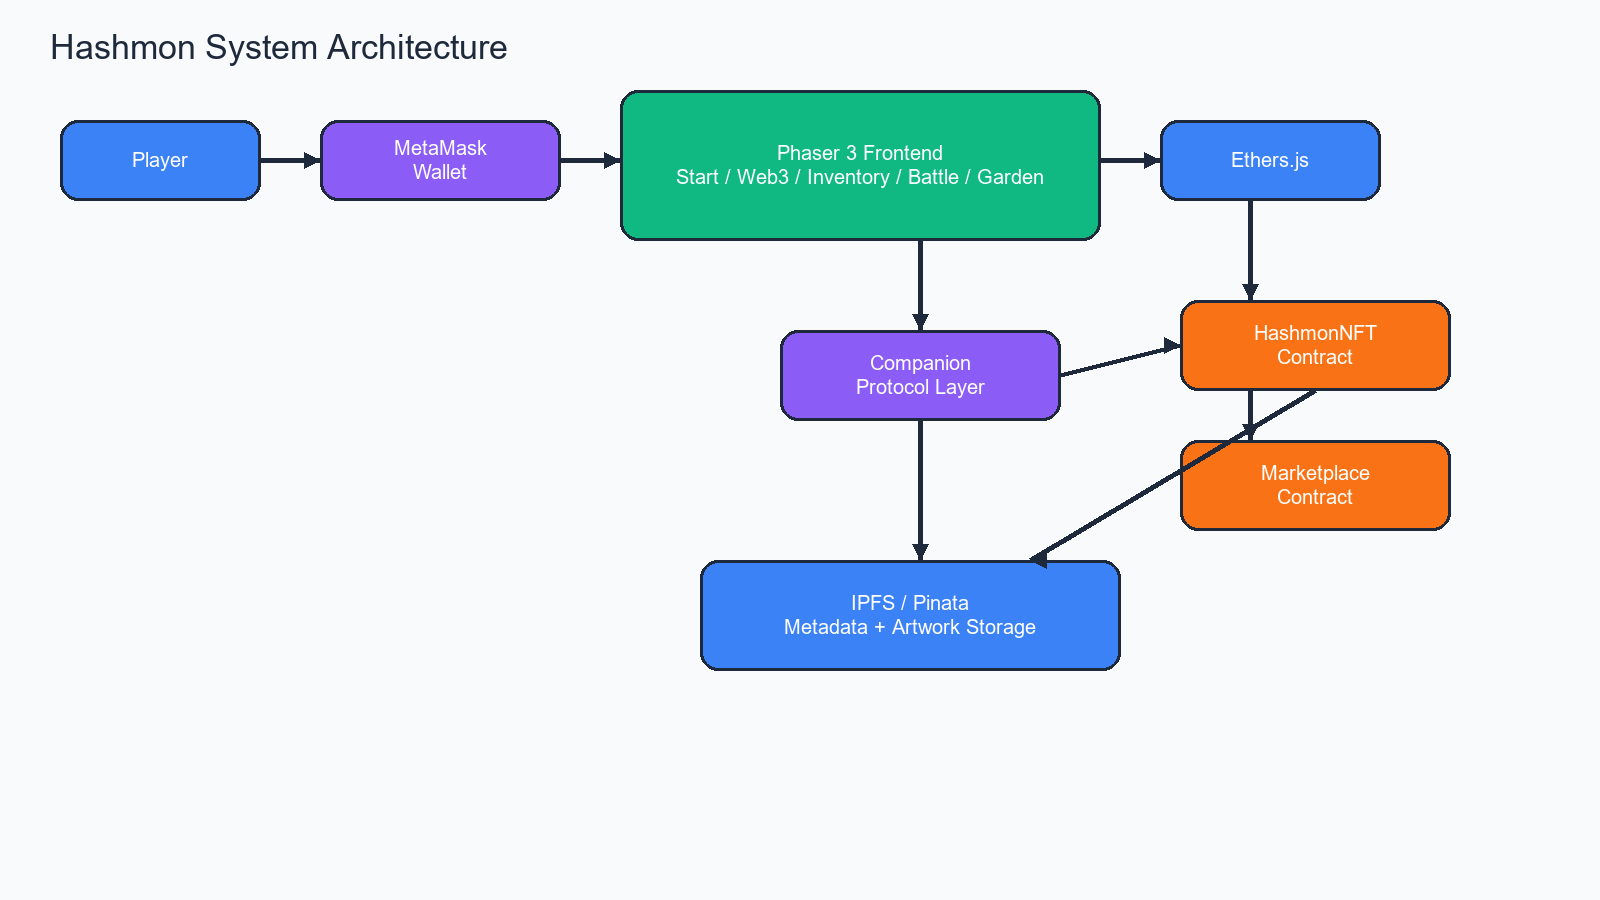
\includegraphics[width=0.9\textwidth]{graphs/hashmon_system_architecture.png}
  \caption{Overall system architecture of Hashmon. The four layers communicate through well-defined interfaces: the Presentation layer renders gameplay via Phaser~3, the Integration layer handles wallet interactions through MetaMask and Ethers.js, the Blockchain layer manages ERC-721 minting and marketplace logic on Sepolia, and the Storage layer persists metadata and artwork on IPFS.}
  \label{fig:architecture}
\end{figure*}

\textbf{Presentation Layer.} The Phaser~3 application layer renders all gameplay interfaces and manages scene transitions. The main scenes include a start screen, a Web3 hub for wallet operations, an inventory view for owned companions, a turn-based battle scene, and a garden scene.

\textbf{Integration Layer.} MetaMask and Ethers.js~v6 act as the bridge between the browser frontend and the Ethereum network. This layer handles wallet connection, transaction signing, contract reads, and event listening. It shields the game logic from low-level blockchain details.

\textbf{Blockchain Layer.} Two Solidity smart contracts, built on OpenZeppelin~\cite{openzeppelin}, manage the asset lifecycle. The \texttt{HashmonNFT} contract handles ERC-721 minting and token metadata URI binding, while the \texttt{HashmonMarketplace} contract supports listing, browsing, and purchase of tokenized companions on the Sepolia testnet.

\textbf{Storage Layer.} Metadata JSON and companion artwork are stored on IPFS using Pinata as a pinning service~\cite{benet2014ipfs}. This ensures that the companion's rich descriptive content remains content-addressed and externally retrievable, independent of the game frontend's runtime state.

A key design element that cuts across all layers is the \emph{Companion Protocol} layer. This protocol standardizes identity information (token ID, nickname, species, type) and portable attributes (agility, vitality, speed, interaction state). By exposing a shared subset of meaning, the protocol allows different gameplay scenes to interpret the same NFT consistently while applying their own mechanics.

\begin{table}[t]
  \caption{Core components of the Hashmon prototype and their roles.}
  \label{tab:components}
  \centering
  \begin{tabular}{p{0.24\linewidth}p{0.66\linewidth}}
    \toprule
    Component & Primary responsibility \\
    \midrule
    Phaser scenes & Render gameplay interfaces and scene-specific interaction logic \\
    Companion protocol & Normalize NFT identity, stats, and portable state \\
    Player profile layer & Maintain active companion selection and cross-scene state updates \\
    NFT contract & Mint ERC-721 tokens and bind metadata URIs to companions \\
    Marketplace contract & Support listing, browsing, and purchase of tokenized companions \\
    IPFS storage & Persist artwork and metadata outside a centralized game database \\
    \bottomrule
  \end{tabular}
\end{table}

This separation of concerns proved useful during implementation. The frontend could evolve rapidly at the scene level without changing the blockchain interface each time, while the protocol layer acted as a stable bridge between the wallet-derived NFT data and the needs of each gameplay module. As a result, the project maintained a relatively clean architecture despite integrating both game logic and Web3 functionality.

\begin{figure*}[!tbp]
  \centering
  \begin{subfigure}{0.48\textwidth}
    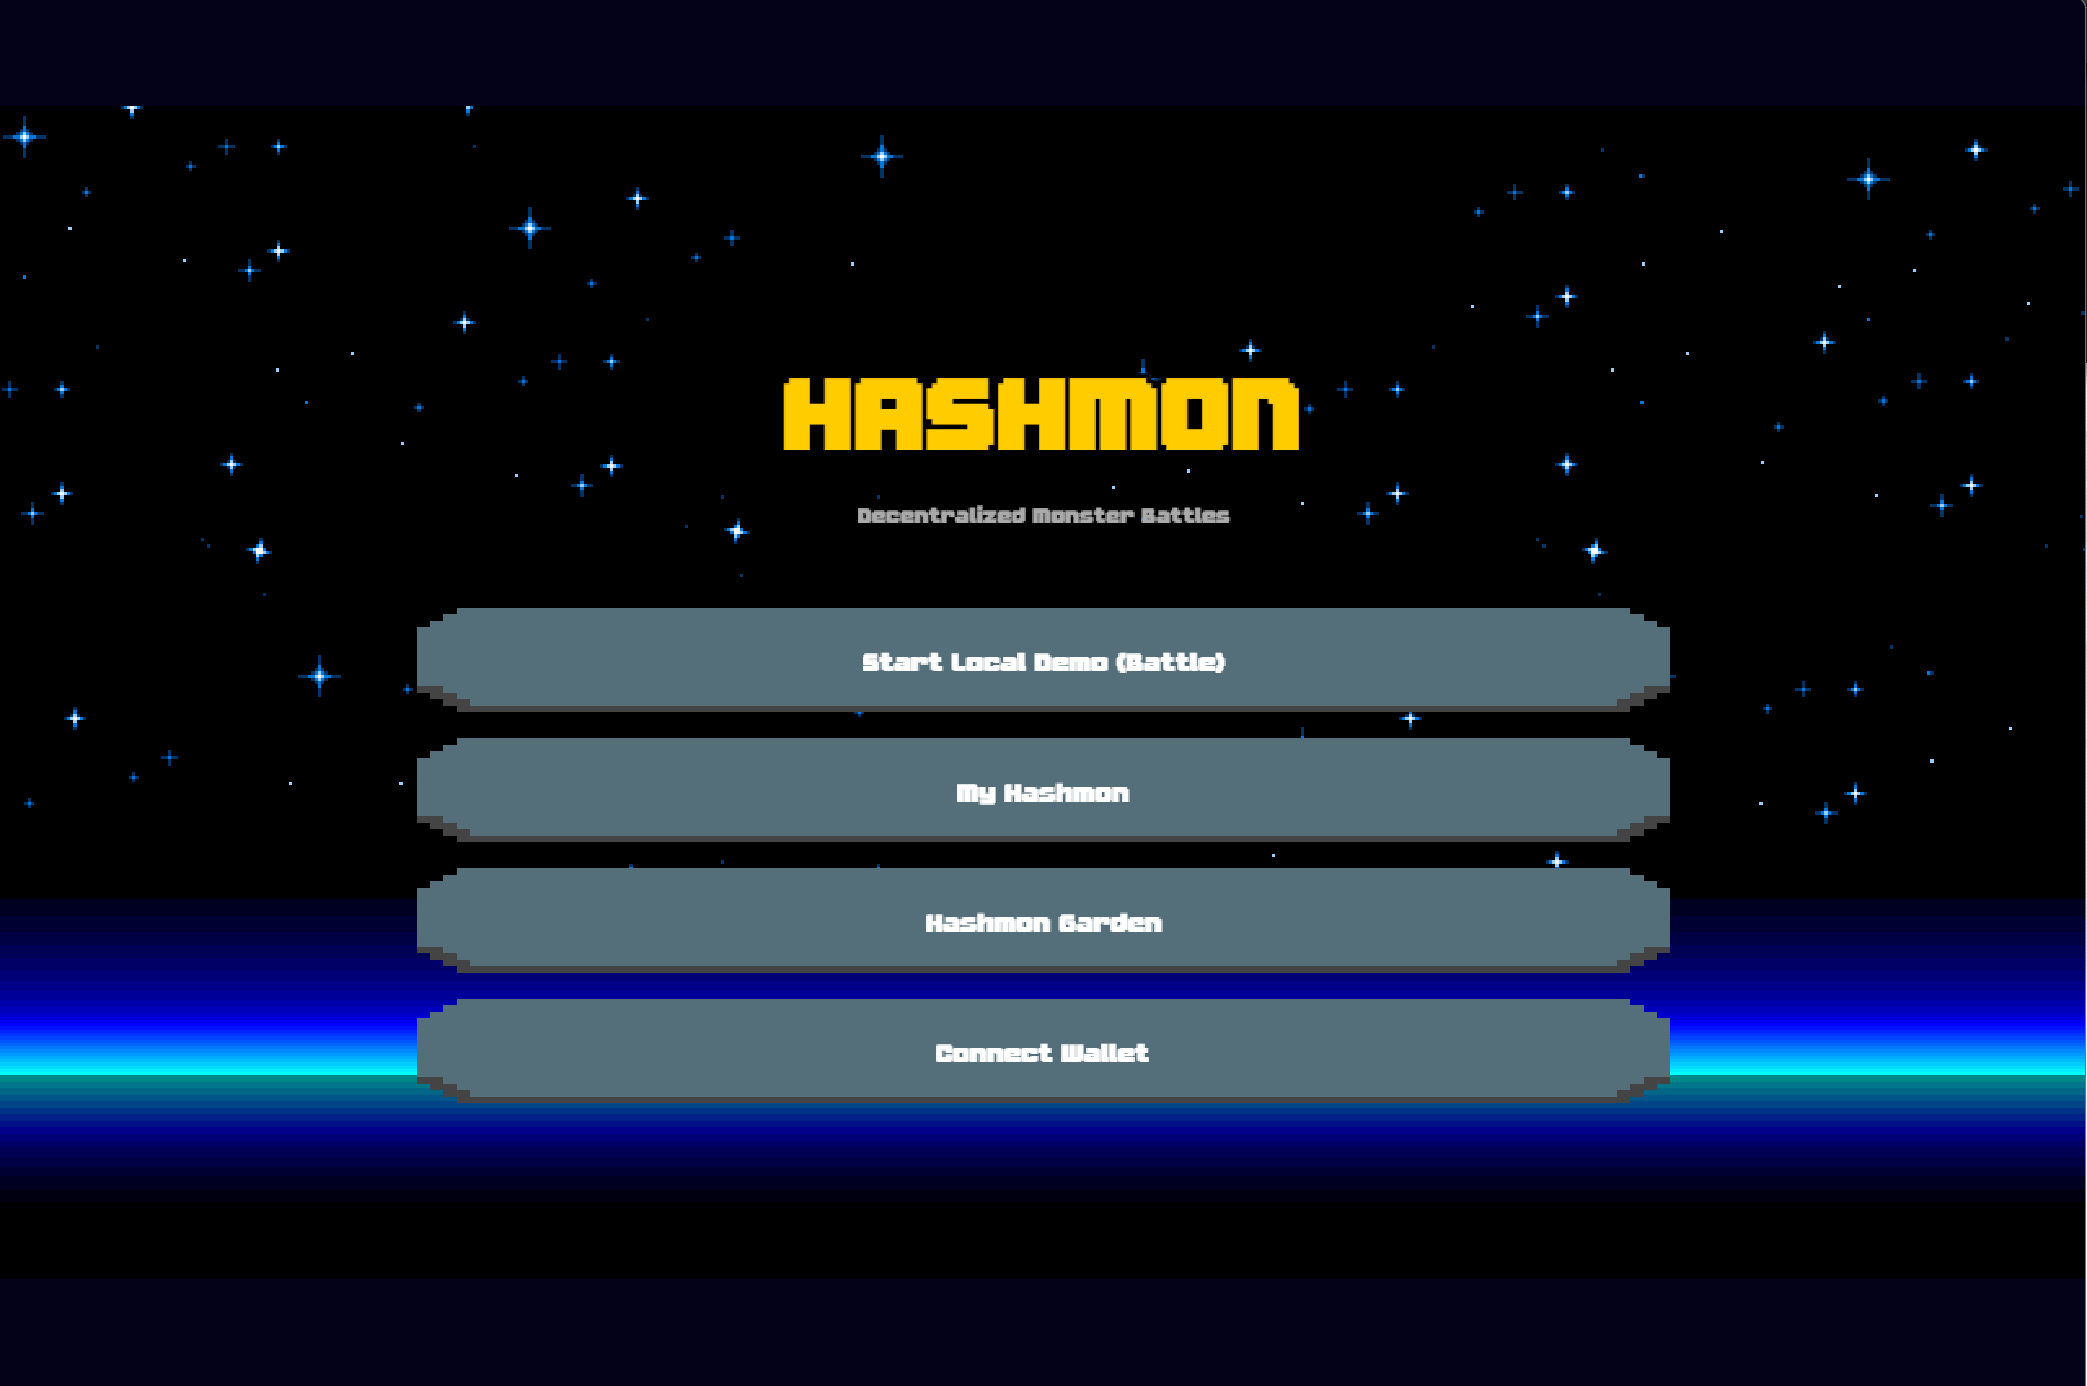
\includegraphics[width=\linewidth]{HomeScene.png}
    \caption{Game home scene and navigation entry points.}
  \end{subfigure}
  \hfill
  \begin{subfigure}{0.48\textwidth}
    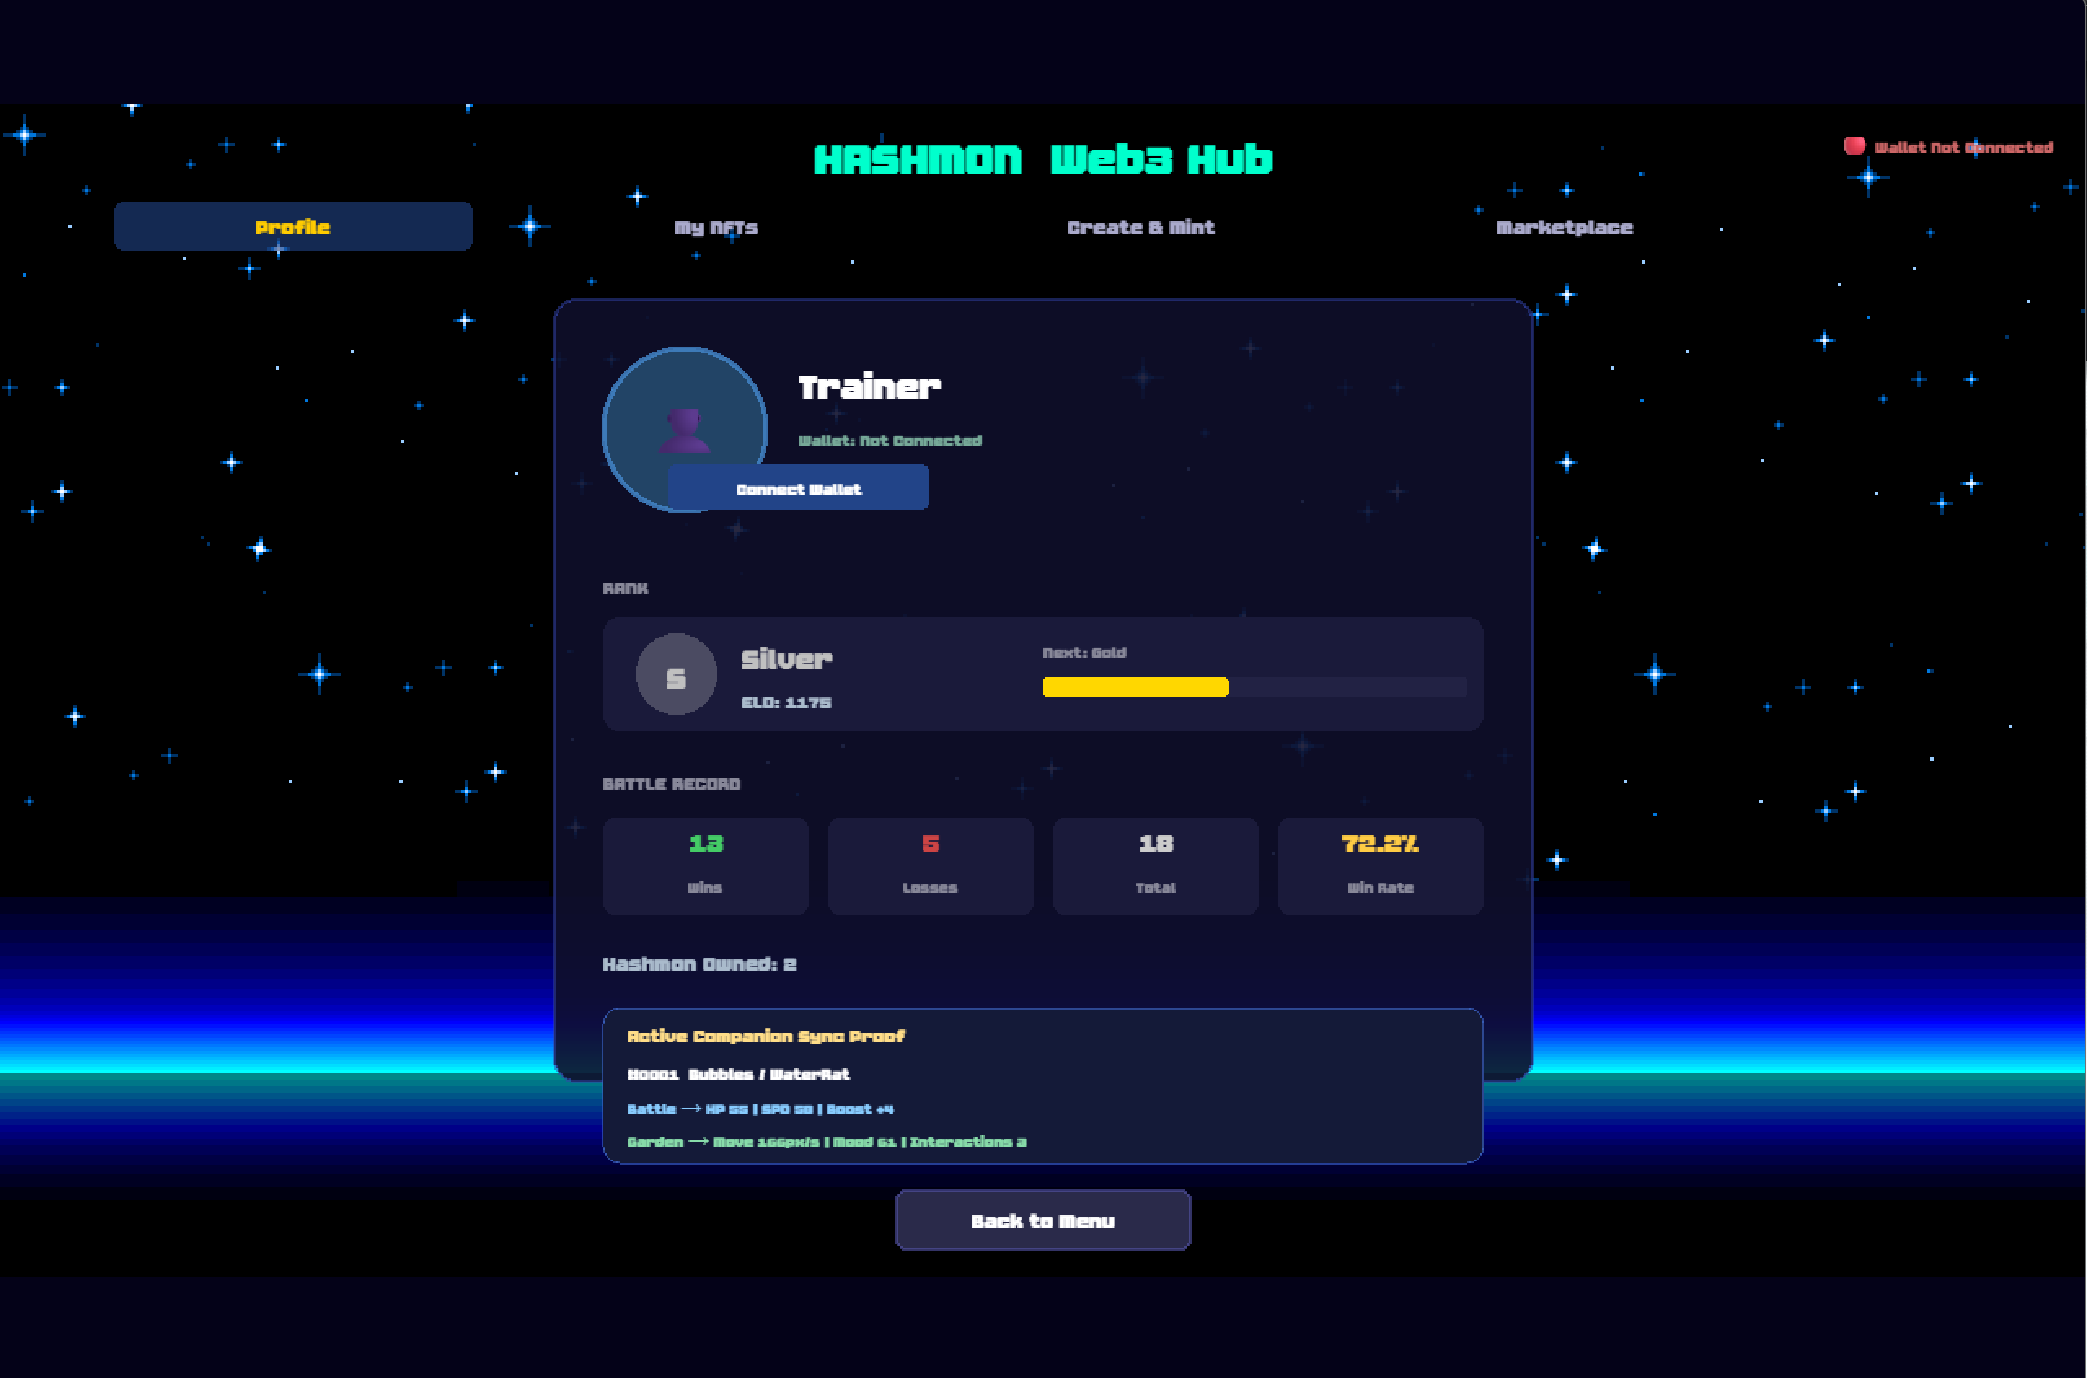
\includegraphics[width=\linewidth]{ConnectwalletScene.png}
    \caption{Web3 wallet entry page.}
  \end{subfigure}

  \vspace{0.6em}

  \begin{subfigure}{0.48\textwidth}
    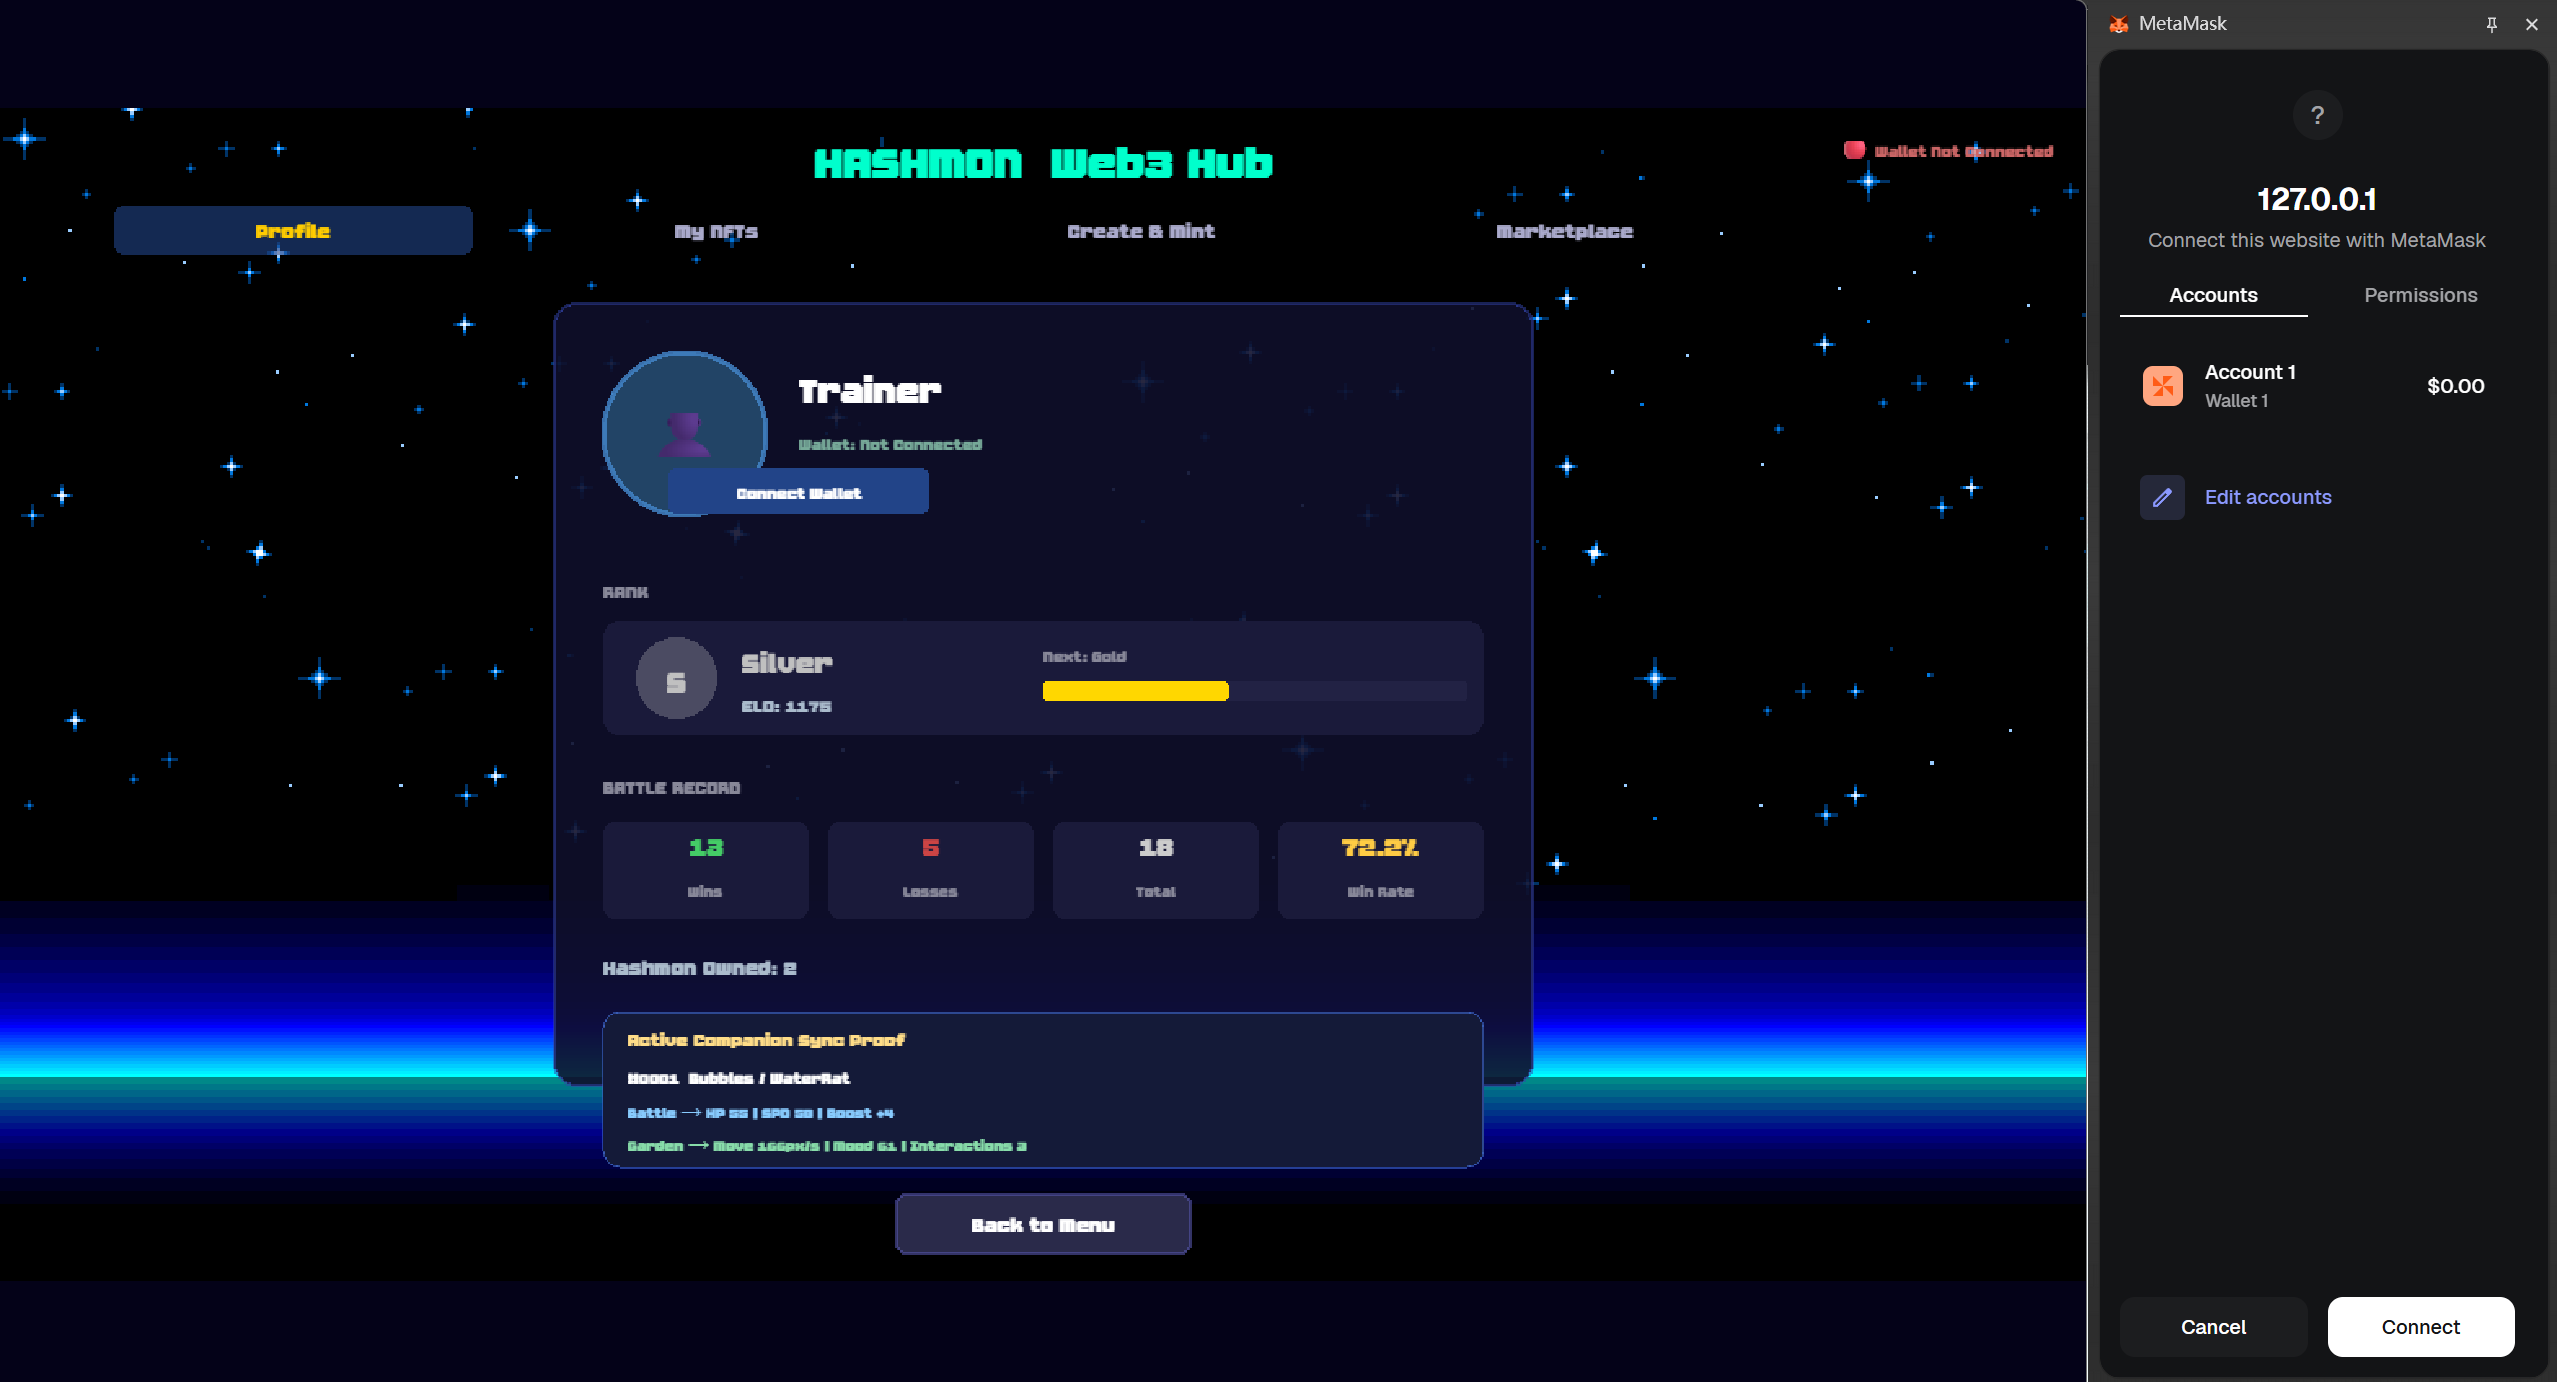
\includegraphics[width=\linewidth]{ConnectwithMetaMask.png}
    \caption{MetaMask authorization interface.}
  \end{subfigure}
  \hfill
  \begin{subfigure}{0.48\textwidth}
    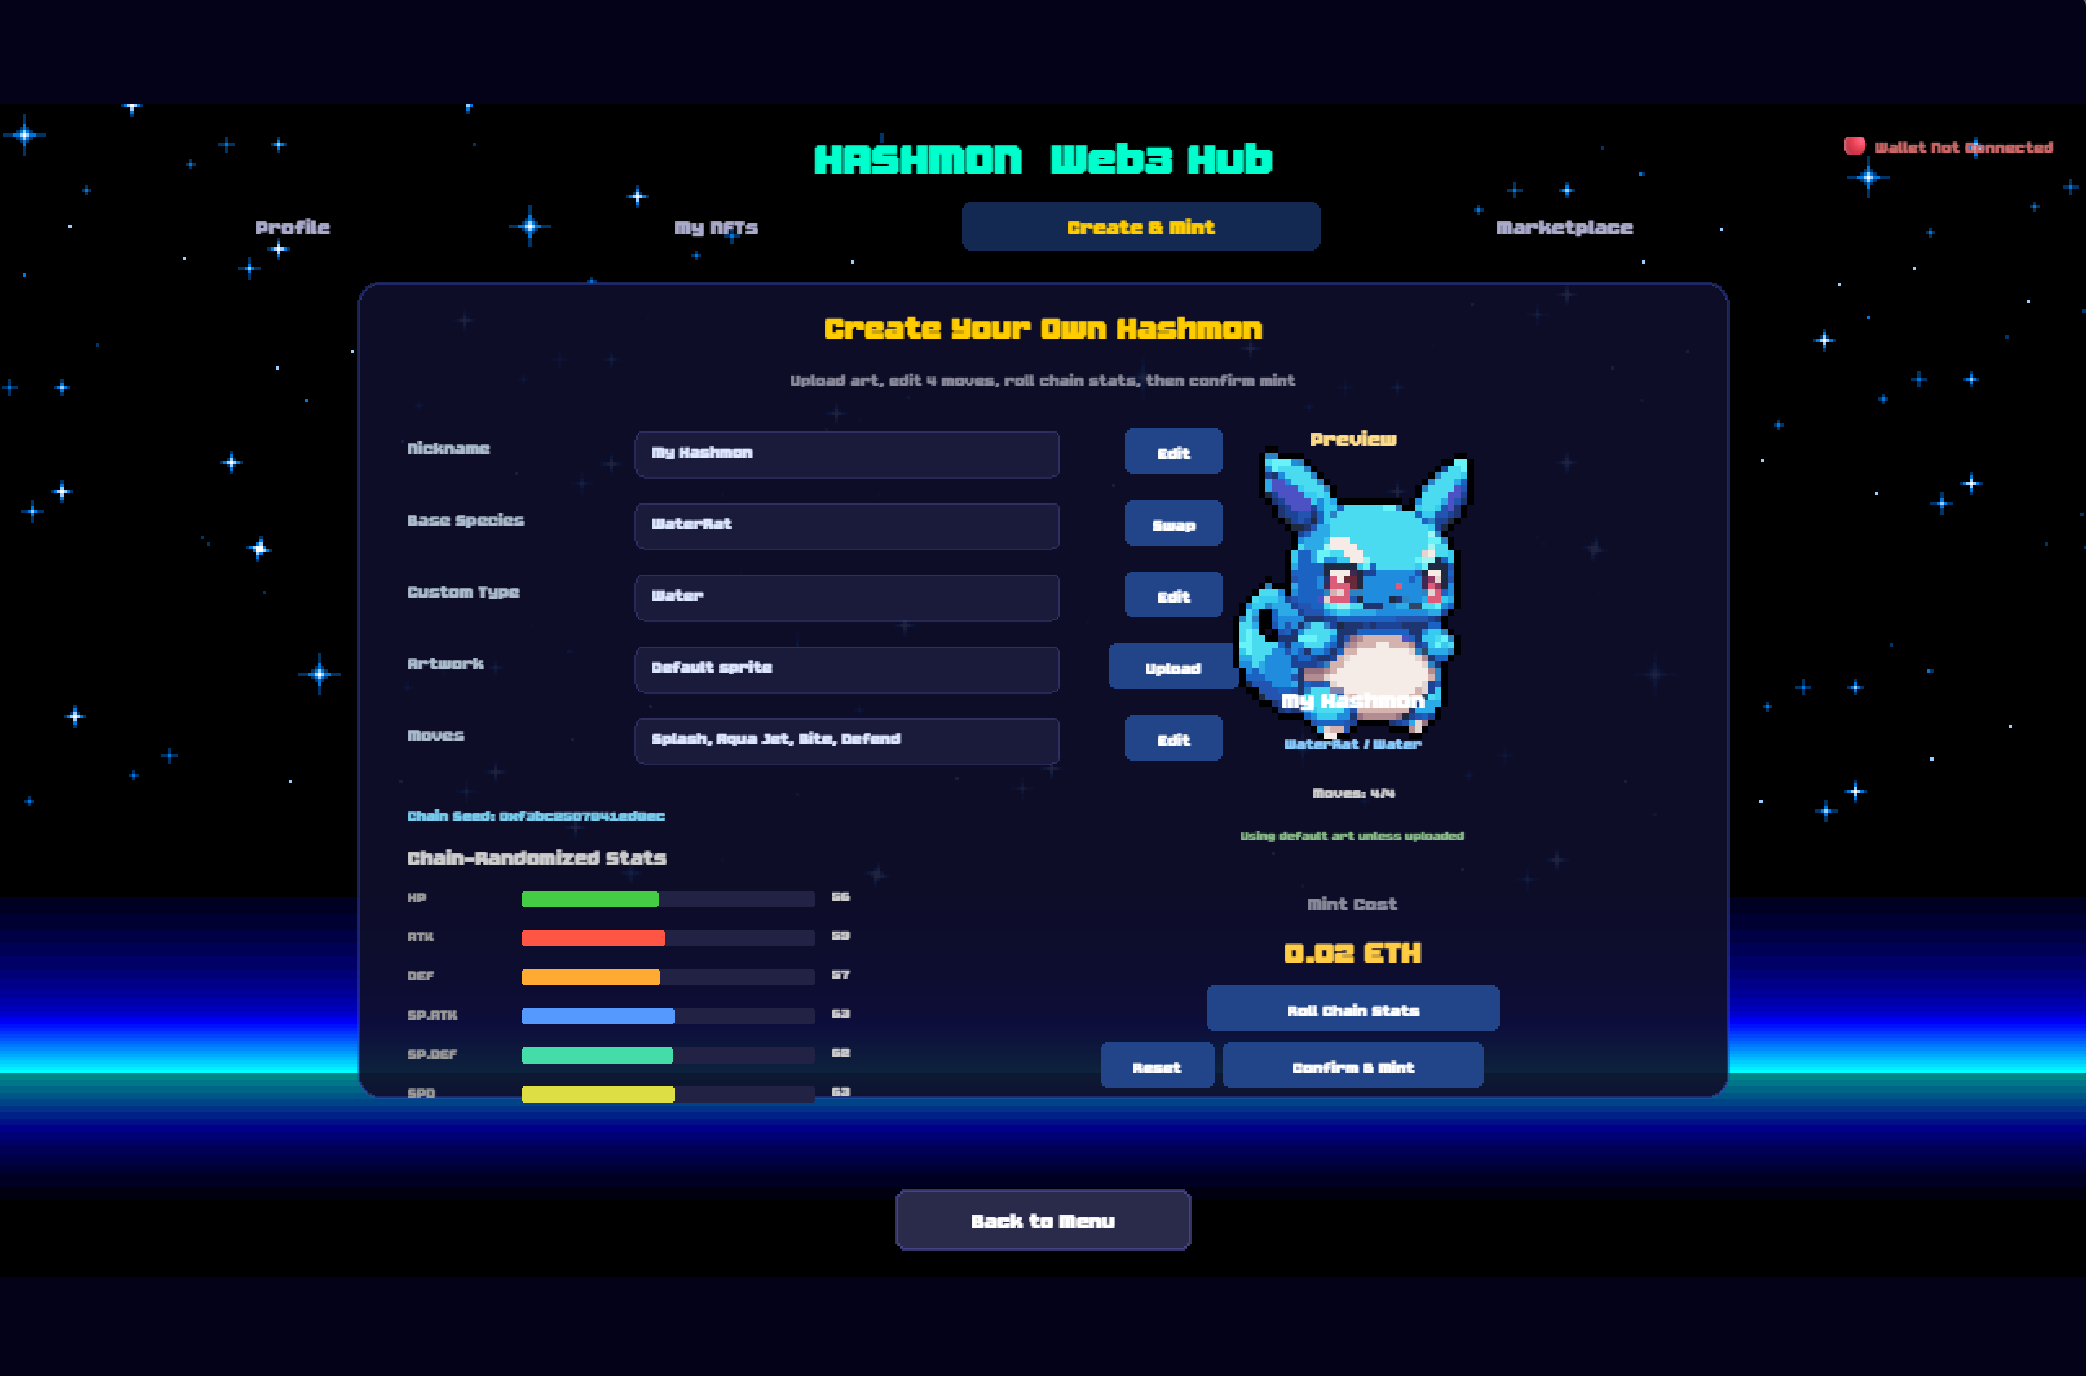
\includegraphics[width=\linewidth]{CreateMint.png}
    \caption{Create-and-mint panel for customized companions.}
  \end{subfigure}
  \caption{Core frontend interfaces of the Hashmon prototype, from game entry to wallet-based creation.}
  \label{fig:ui-overview}
\end{figure*}

The user interface was designed to make the Web3 workflow visible rather than hidden. Players can clearly see when they are entering the wallet flow, when they are defining companion metadata, and when the asset becomes available inside the game world. This transparency is useful in both a teaching context and a prototype evaluation context.

\section{Workflow and Implementation}
The end-to-end user workflow follows a \emph{pipeline-then-fan-out} pattern. In the pipeline stage, a companion is designed, uploaded to IPFS, minted as an ERC-721 token, and synchronized to the player's wallet. In the fan-out stage, the same NFT-backed companion is distributed to three independent game contexts: battle, garden, and marketplace. This architecture ensures that a single companion is created once, owned cryptographically, and reused across all scenes without duplication.

\subsection{Pipeline: Wallet Connection and Minting}
The pipeline begins when a player connects MetaMask in the Web3 hub. After wallet connection, the frontend queries the NFT contract for owned token IDs and token URIs, resolves metadata through IPFS, and reconstructs the in-game representation of each Hashmon.

Users can then create a new companion by specifying nickname, species, type, moves, and optional custom artwork. The application uploads the artwork and metadata to IPFS and finally calls the mint function on the Sepolia NFT contract. This creates a full browser-to-chain minting pipeline, as illustrated in Figures~\ref{fig:wallet-mint} and~\ref{fig:ownership-views}.

\begin{figure*}[!tbp]
  \centering
  \begin{subfigure}{0.48\textwidth}
    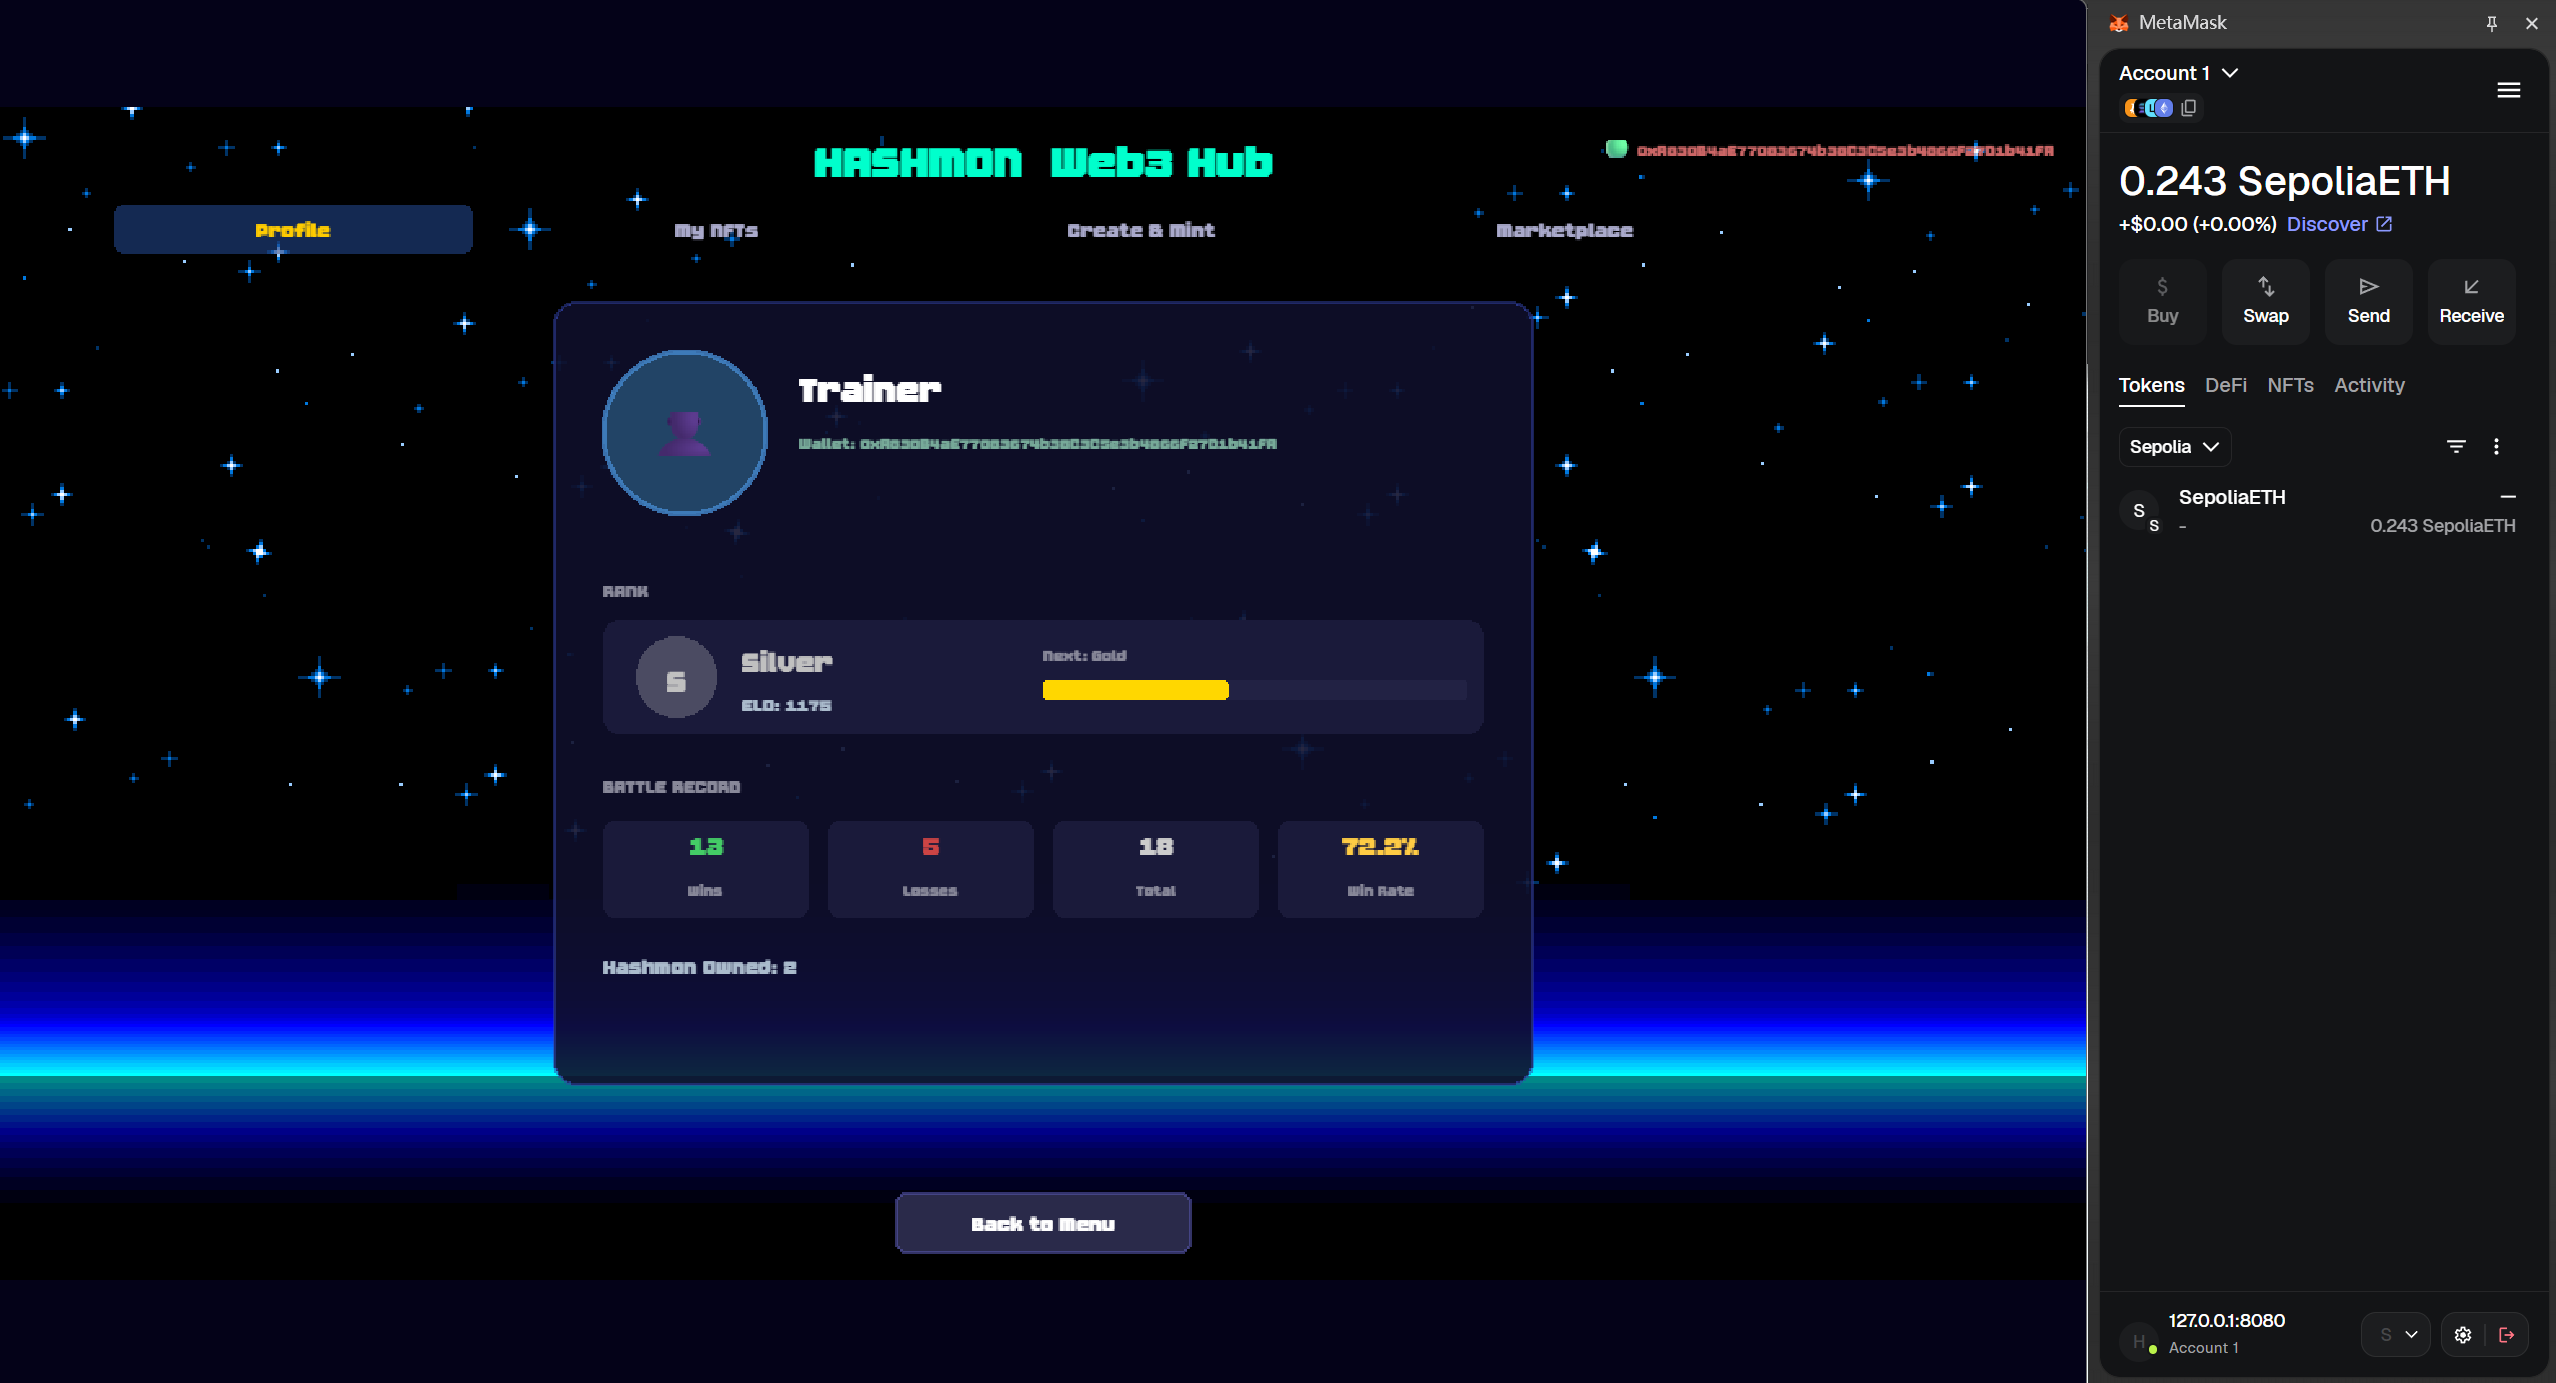
\includegraphics[height=0.22\textheight,keepaspectratio]{ConnectedwithMetaMask.png}
    \caption{Wallet successfully connected to the prototype.}
  \end{subfigure}
  \hfill
  \begin{subfigure}{0.48\textwidth}
    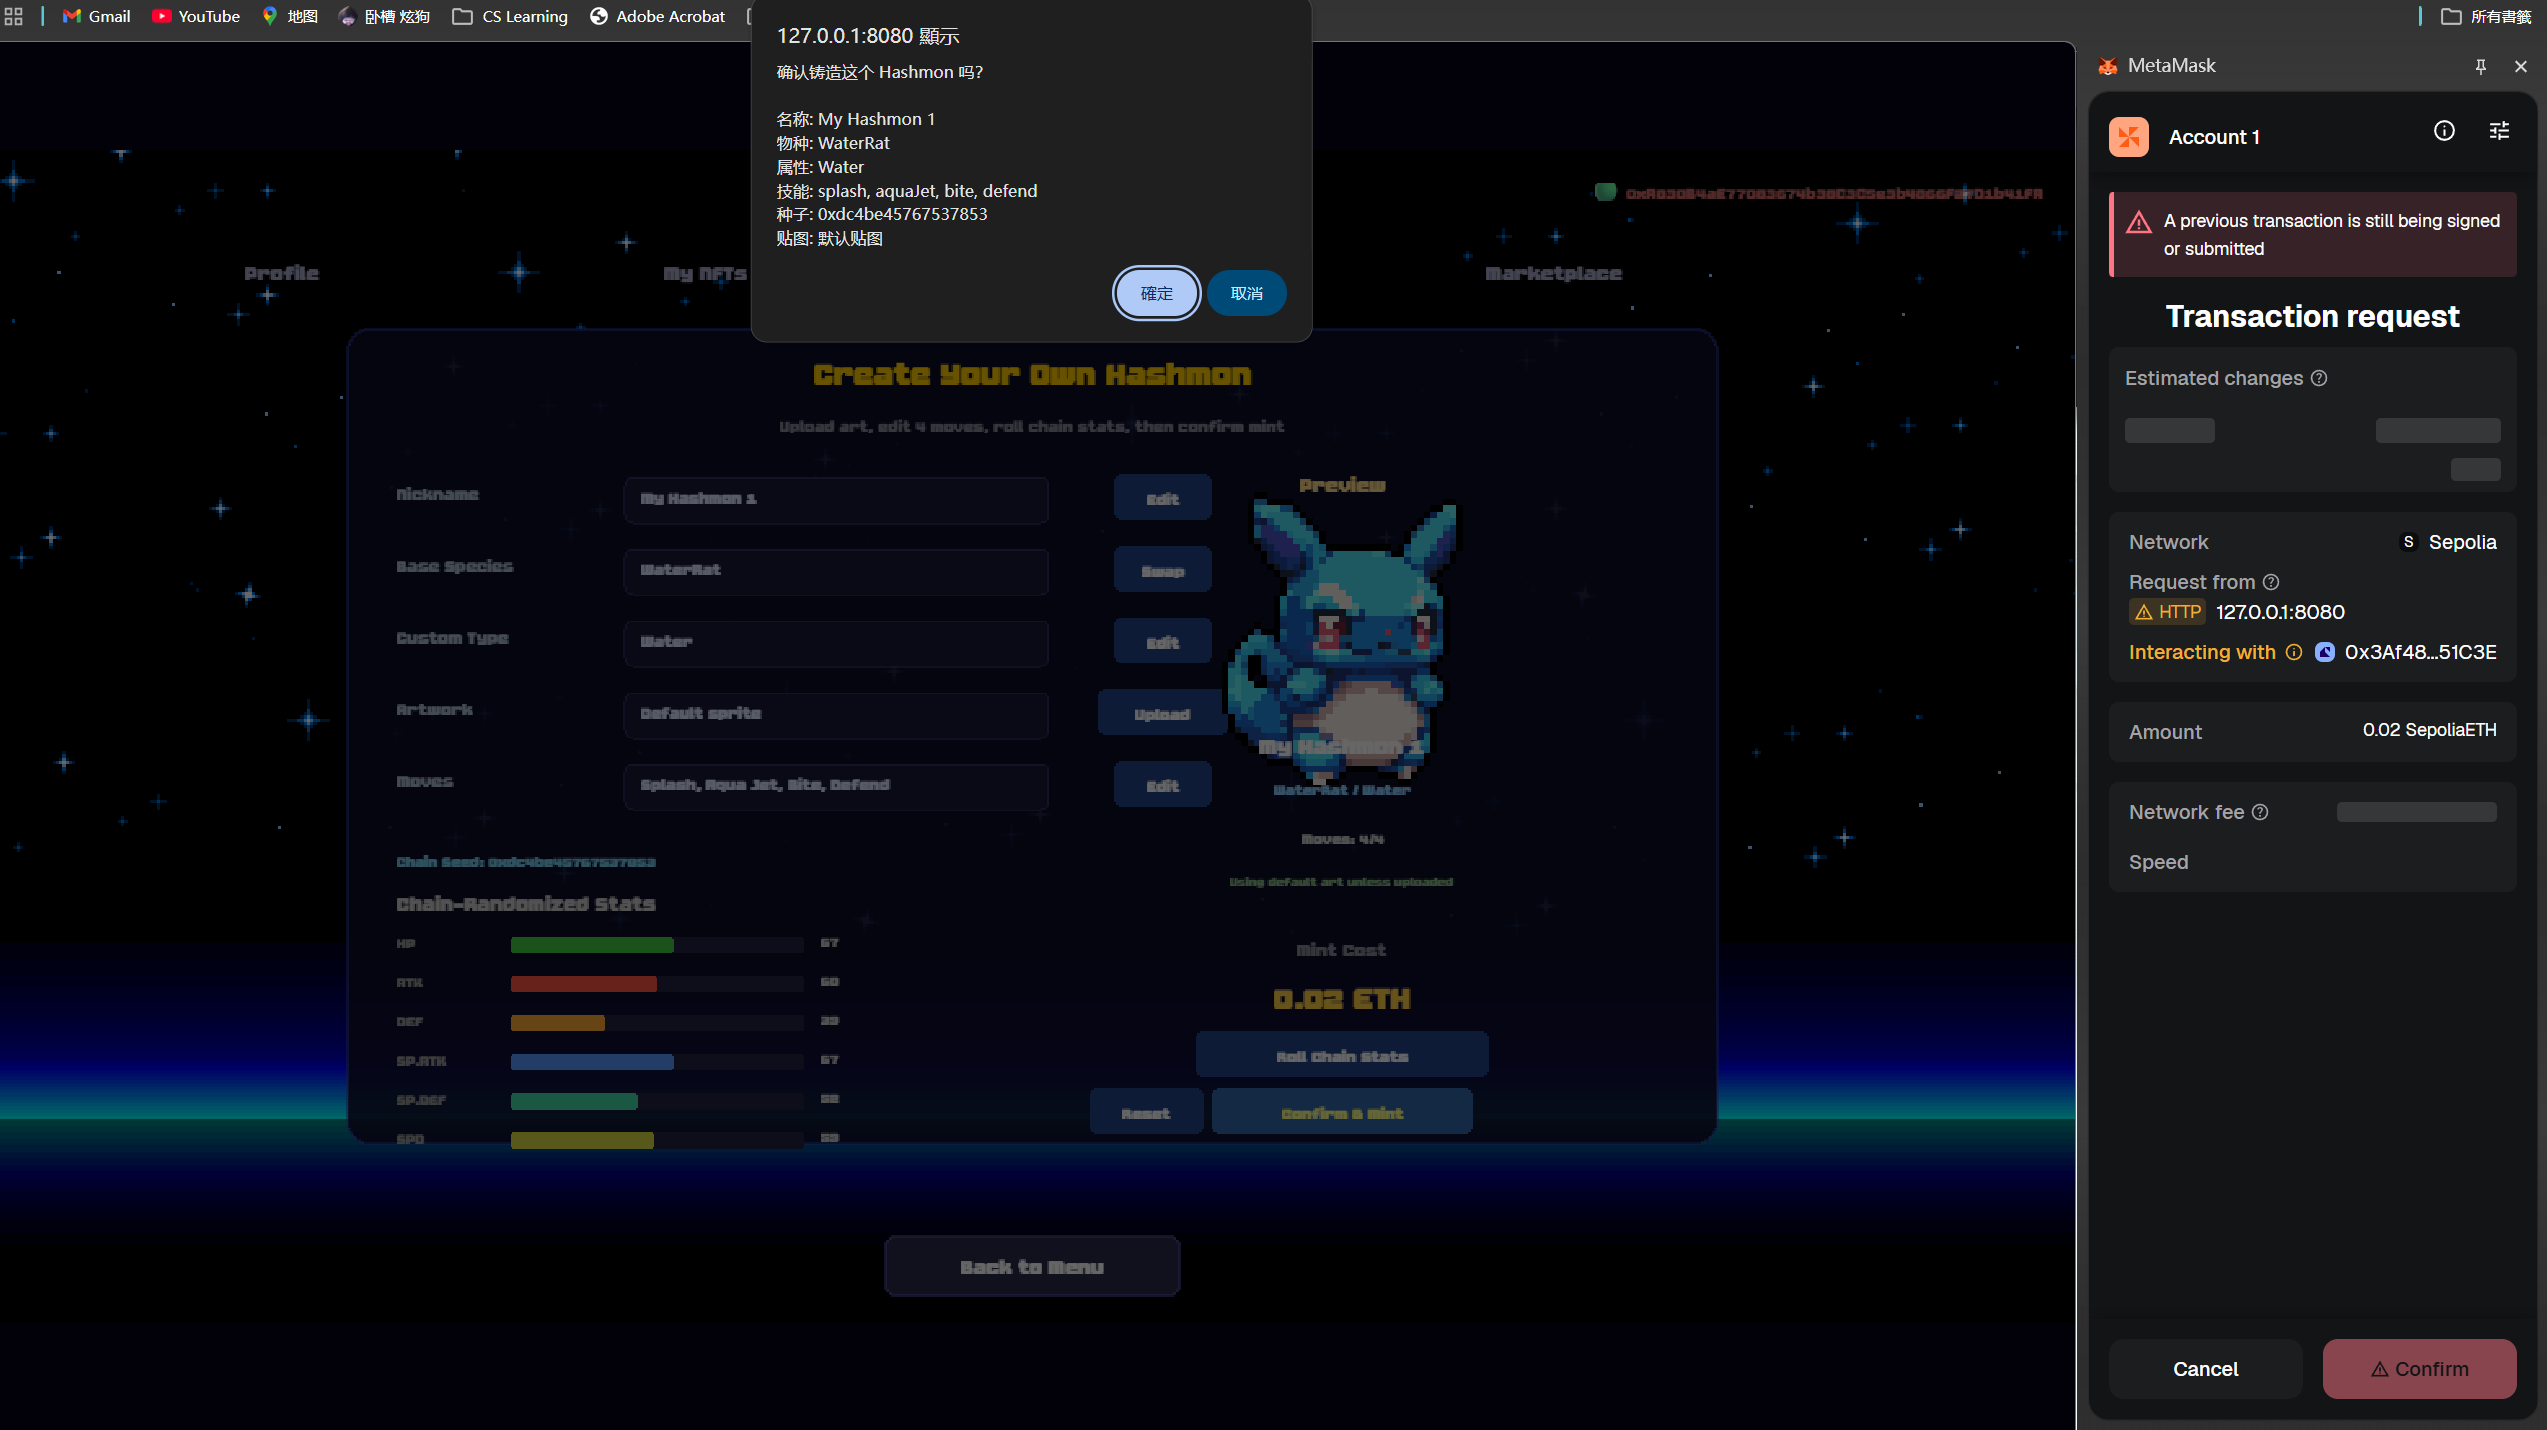
\includegraphics[height=0.22\textheight,keepaspectratio]{MintProcess.png}
    \caption{Mint transaction and upload process.}
  \end{subfigure}

  \vspace{0.6em}

  \begin{subfigure}{0.48\textwidth}
    \includegraphics[height=0.22\textheight,keepaspectratio]{Minted.png}
    \caption{Confirmation that a new Hashmon has been minted.}
  \end{subfigure}
  \hfill
  \begin{subfigure}{0.48\textwidth}
    \centering
    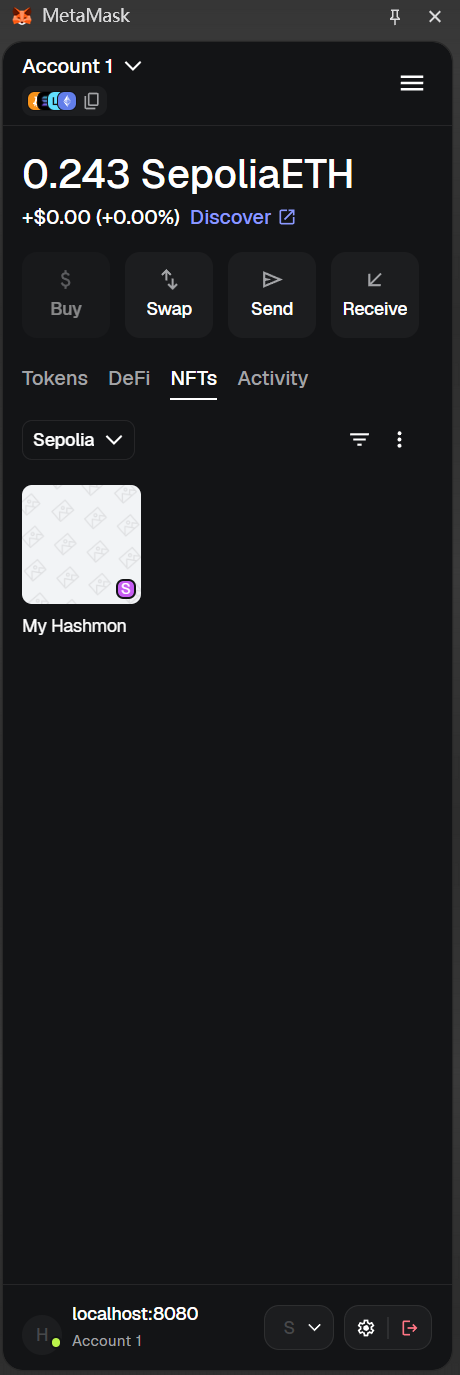
\includegraphics[height=0.22\textheight,keepaspectratio]{NewNFTMintedinwallet.png}
    \caption{The newly minted NFT reflected in the wallet view.}
  \end{subfigure}
  \caption{Wallet connection and mint lifecycle in the Hashmon prototype.}
  \label{fig:wallet-mint}
\end{figure*}

A complete mint cycle is particularly important for demonstrating that the prototype is not a purely visual mock-up. The screenshots show the chain-aware lifecycle of the asset, beginning with wallet authorization and ending with the companion appearing as a user-owned NFT.

\begin{figure*}[!tbp]
  \centering
  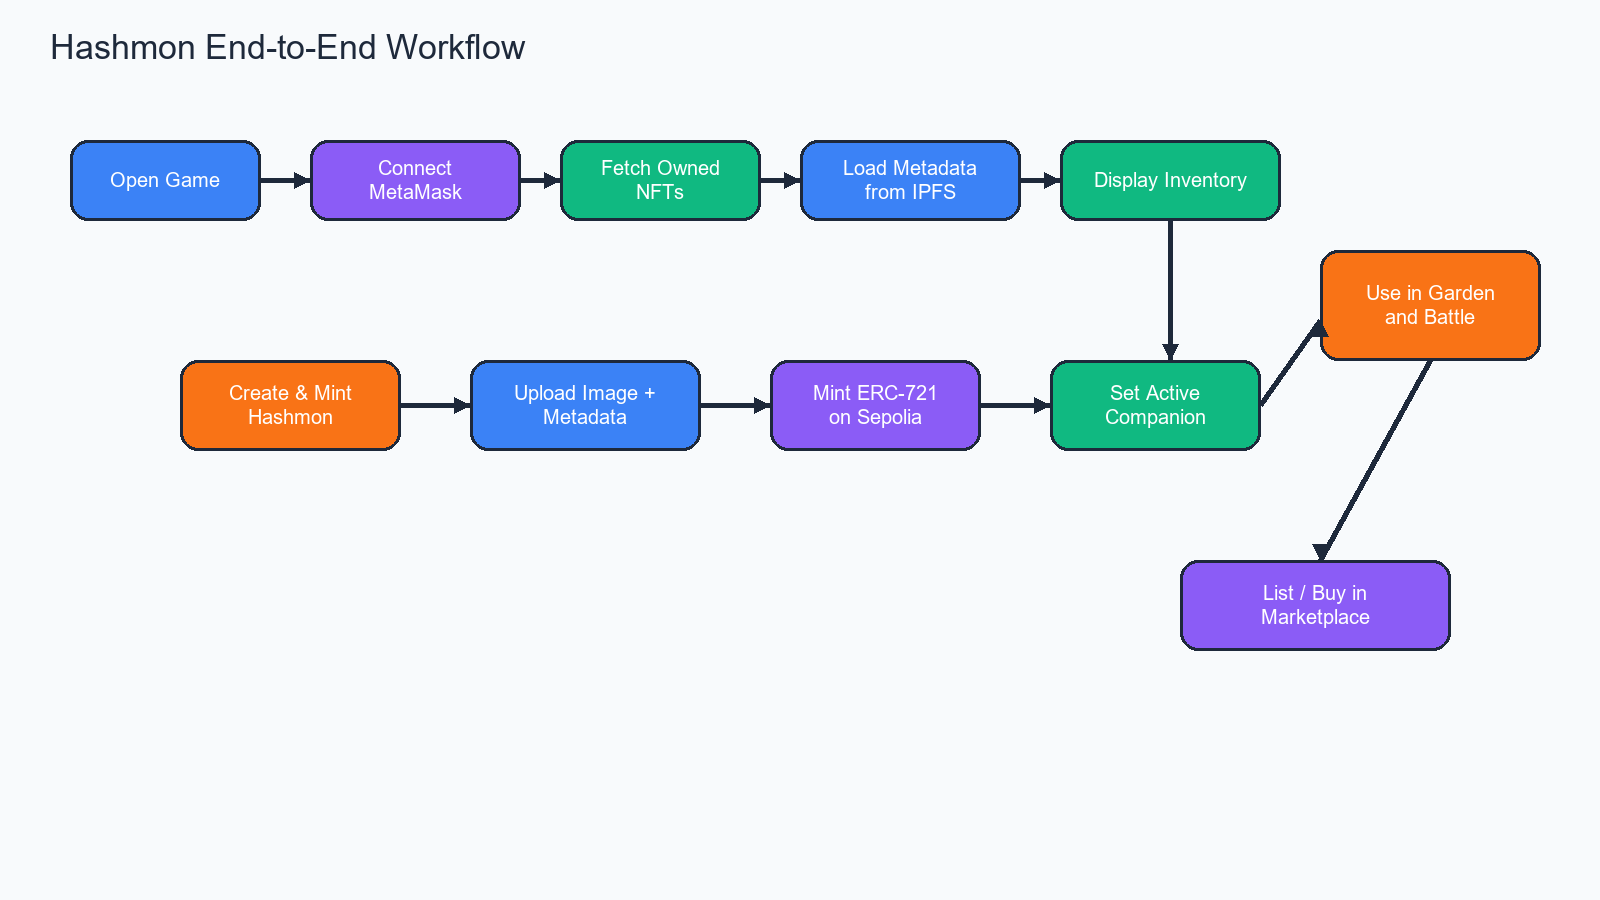
\includegraphics[width=0.92\textwidth]{graphs/hashmon_end_to_end_workflow.png}
  \caption{End-to-end workflow from wallet connection to minting, gameplay reuse, and marketplace trading. The pipeline stage (left-to-right) feeds into a fan-out stage that distributes the companion across battle, garden, and marketplace contexts.}
  \label{fig:workflow}
\end{figure*}

\subsection{Fan-Out: Scene Reuse and Marketplace}
Once a companion is minted and wallet-synchronized, the active companion mechanism allows the player to select one owned NFT as the currently active Hashmon. This active asset is then consumed by the battle, garden, and marketplace modules simultaneously. The marketplace further extends the prototype beyond minting by allowing users to list companions for sale and buy listed NFTs from other wallets. This makes the NFT meaningful not only as a collectible but also as a tradable Web3 game asset with real economic value.

\begin{figure*}[!tbp]
  \centering
  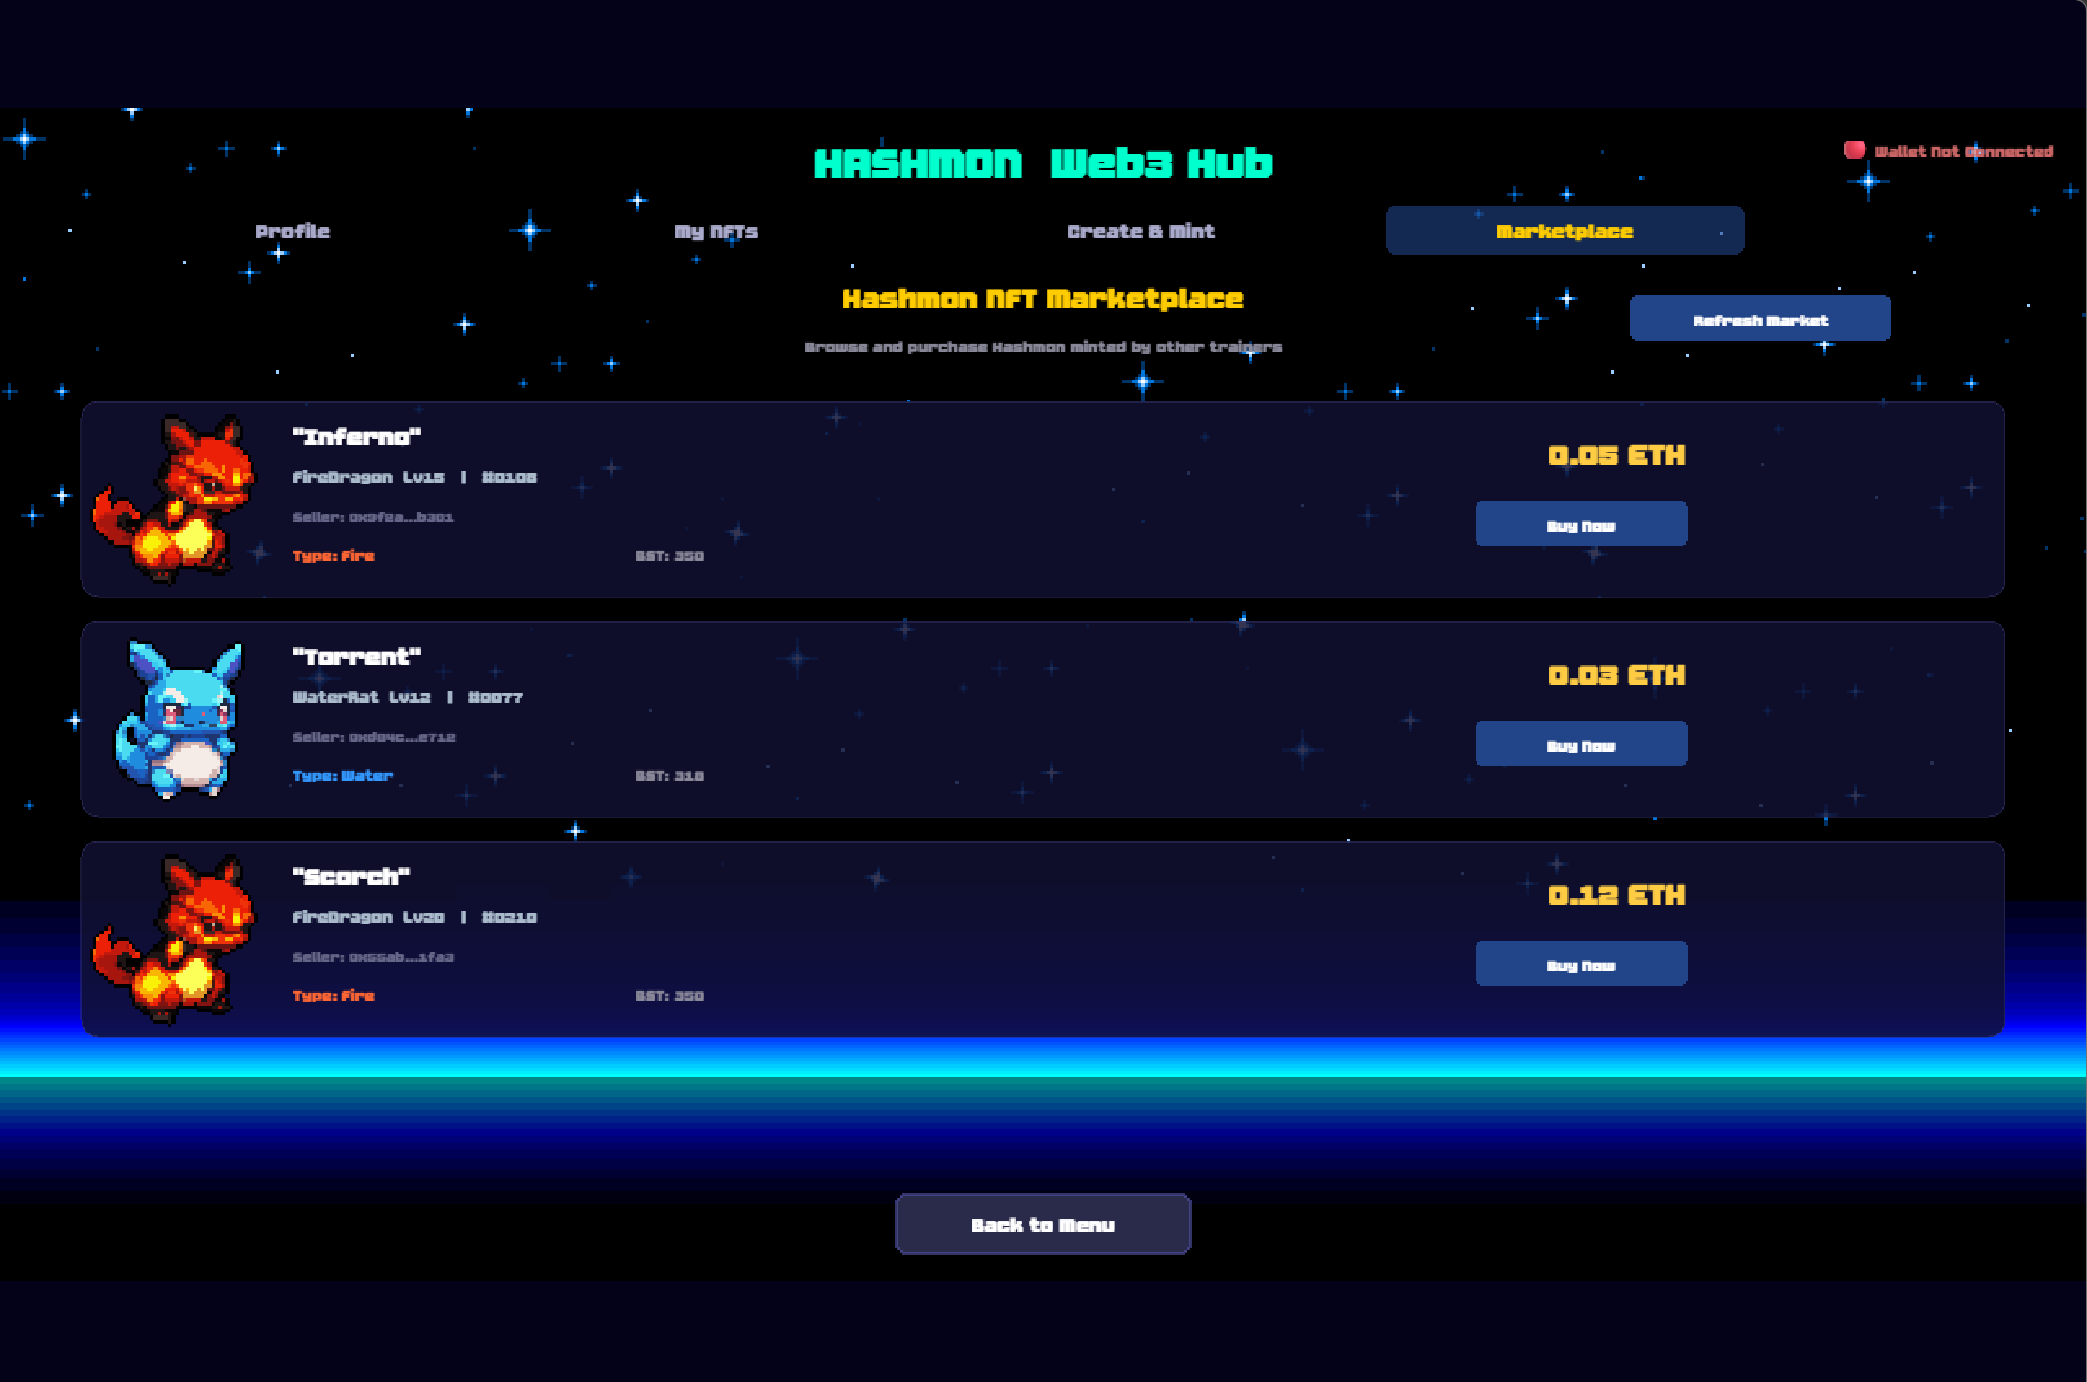
\includegraphics[width=0.78\textwidth,height=0.26\textheight,keepaspectratio]{MarketPlace.png}
  \caption{Integrated marketplace interface showing listed Hashmon NFTs and prices.}
  \label{fig:marketplace}
\end{figure*}

\begin{figure*}[!tbp]
  \centering
  \begin{subfigure}{0.48\textwidth}
    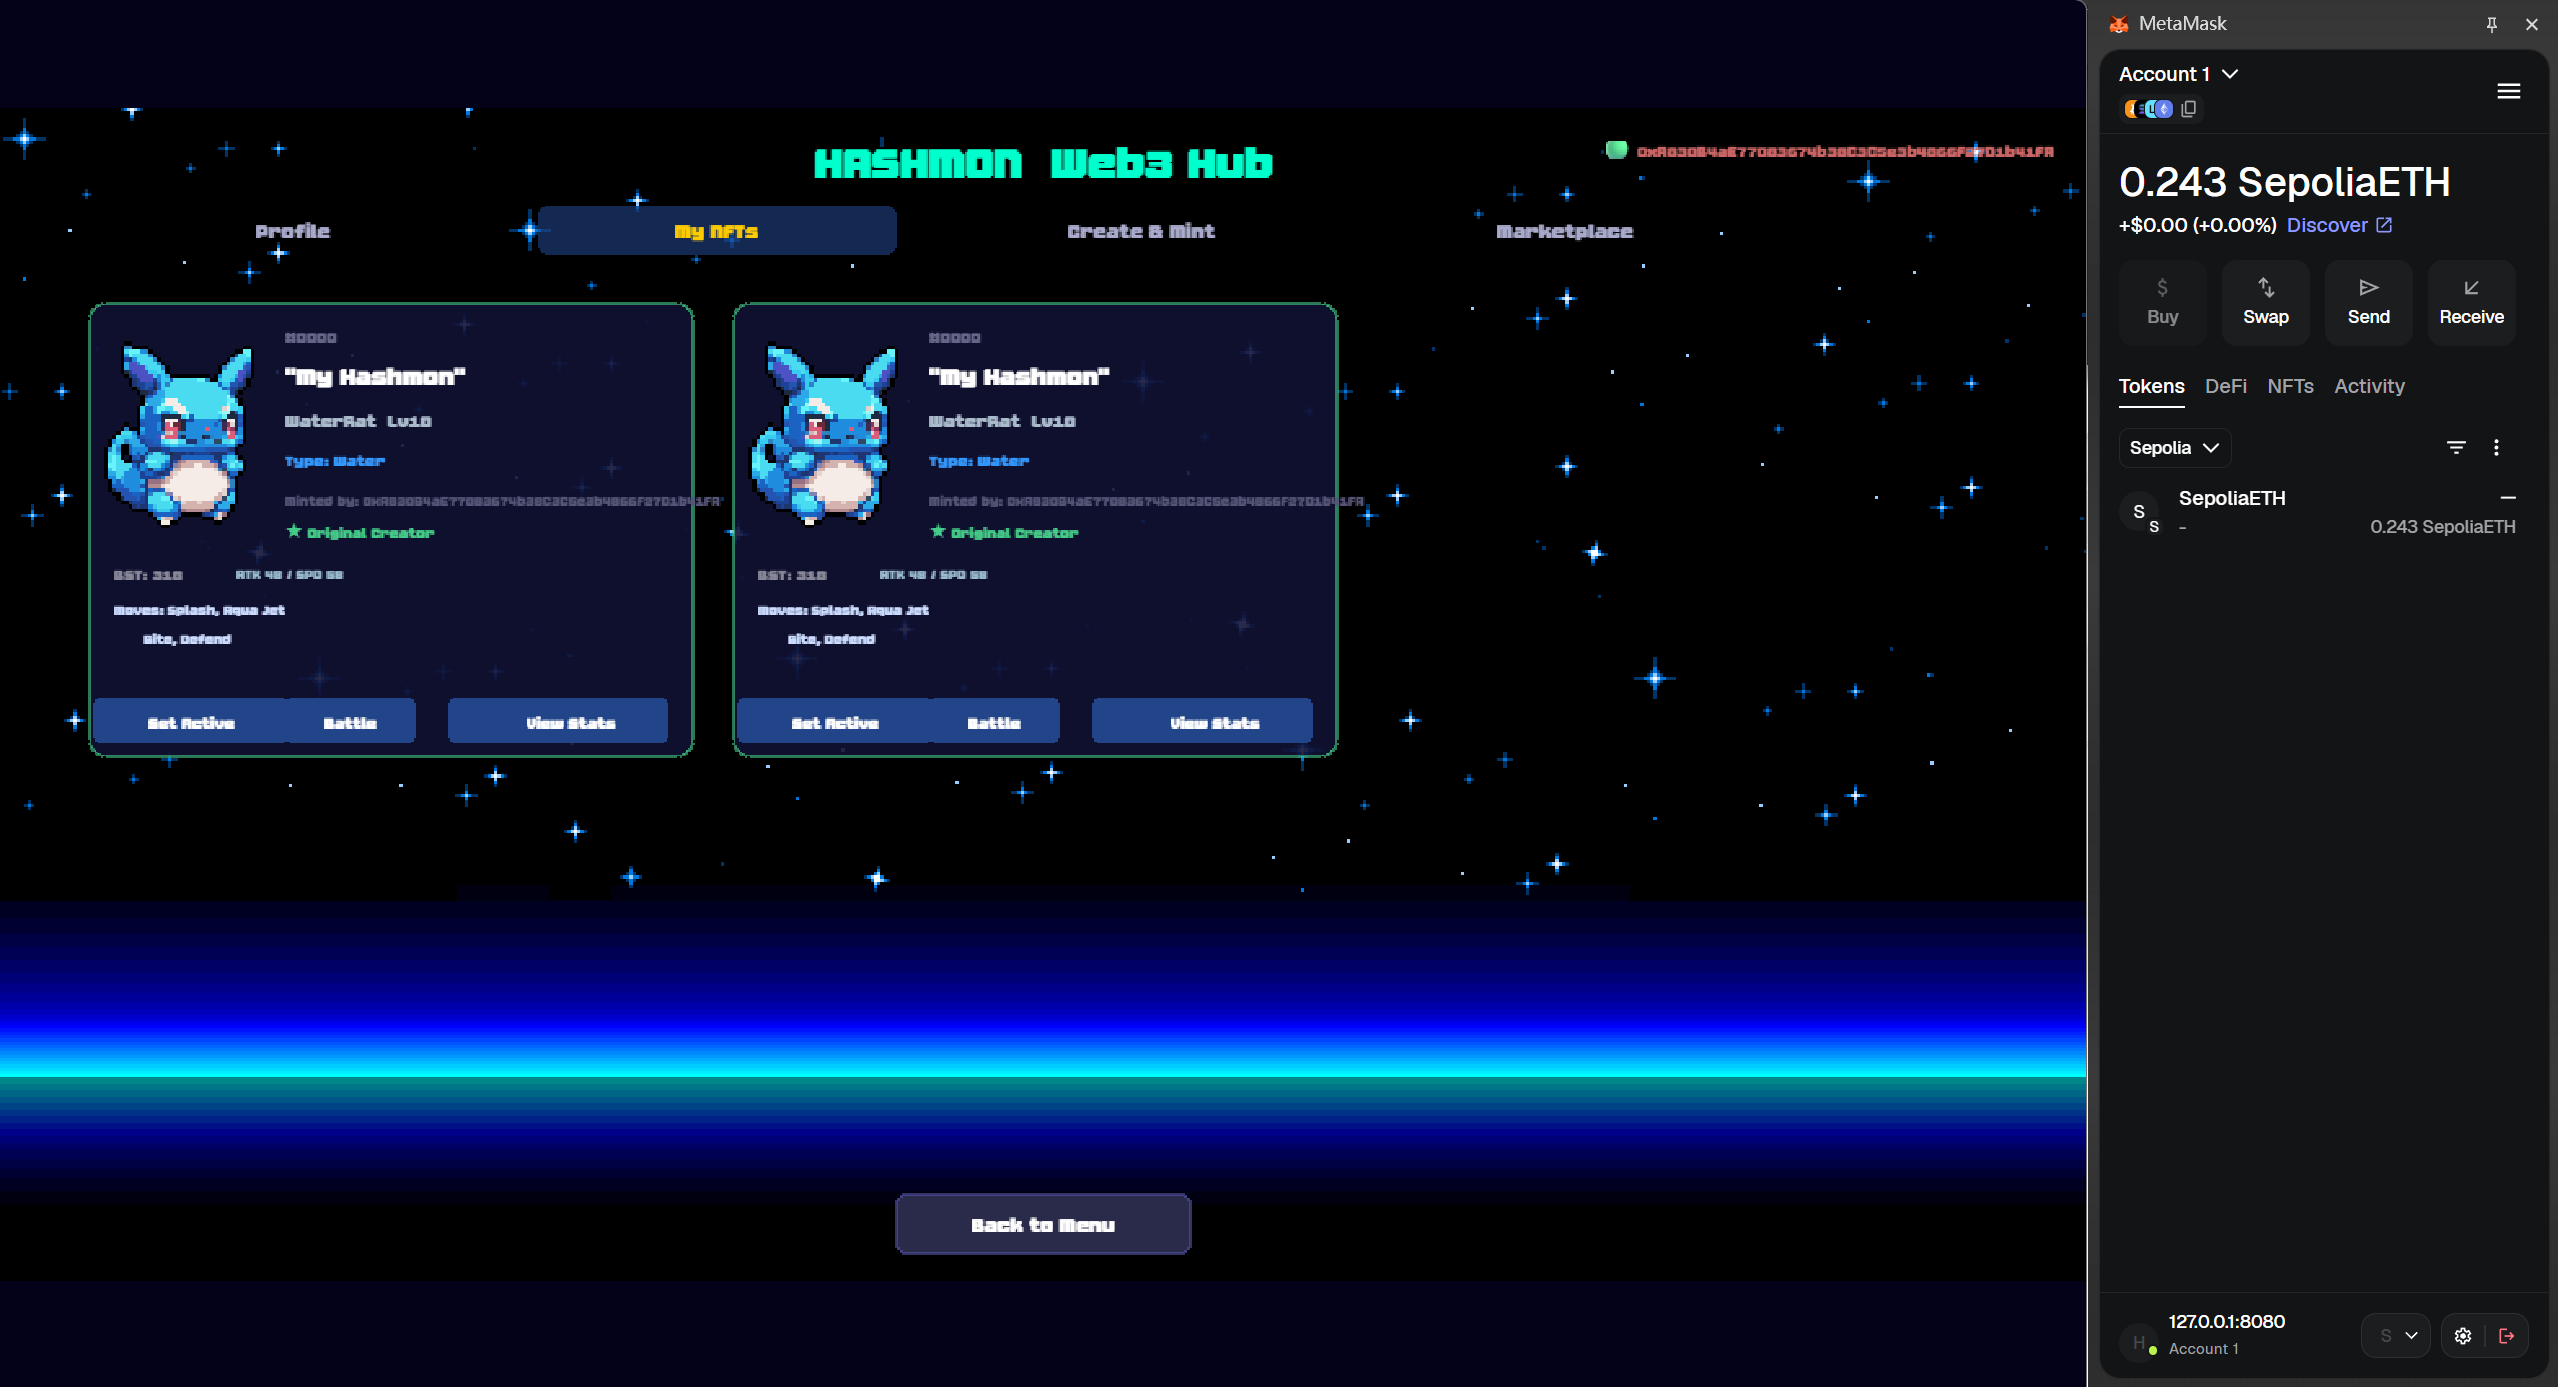
\includegraphics[height=0.22\textheight,keepaspectratio]{HashmonReadfromWallet.png}
    \caption{Reading NFT companion metadata directly from the wallet.}
  \end{subfigure}
  \hfill
  \begin{subfigure}{0.48\textwidth}
    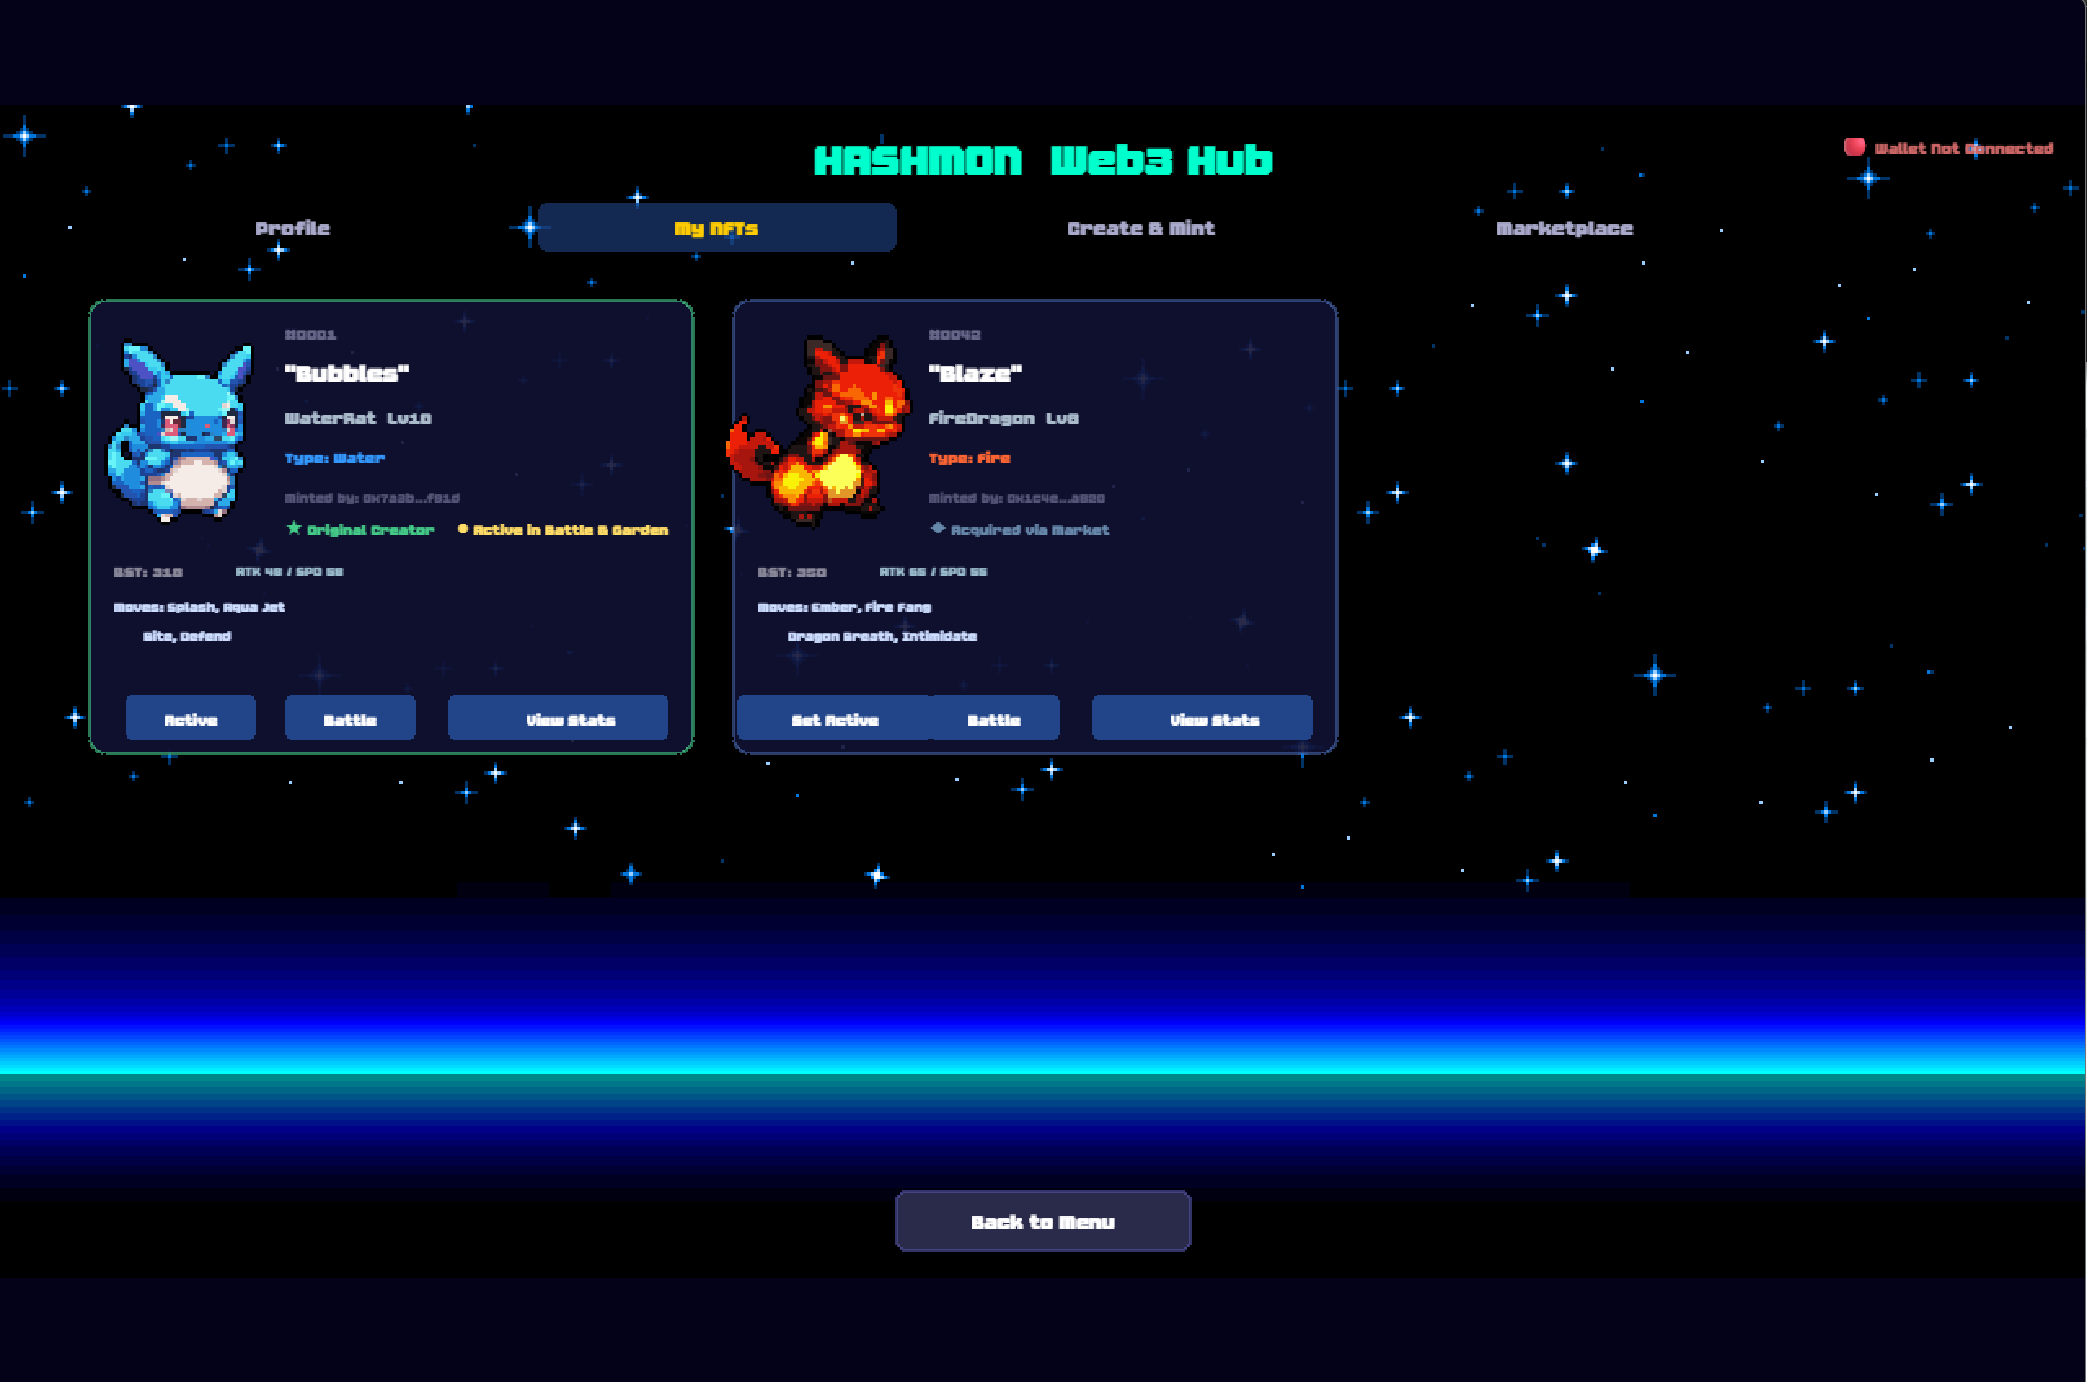
\includegraphics[height=0.22\textheight,keepaspectratio]{MyNFTs.png}
    \caption{Personal NFT inventory view.}
  \end{subfigure}

  \vspace{0.6em}

  \begin{subfigure}{0.48\textwidth}
    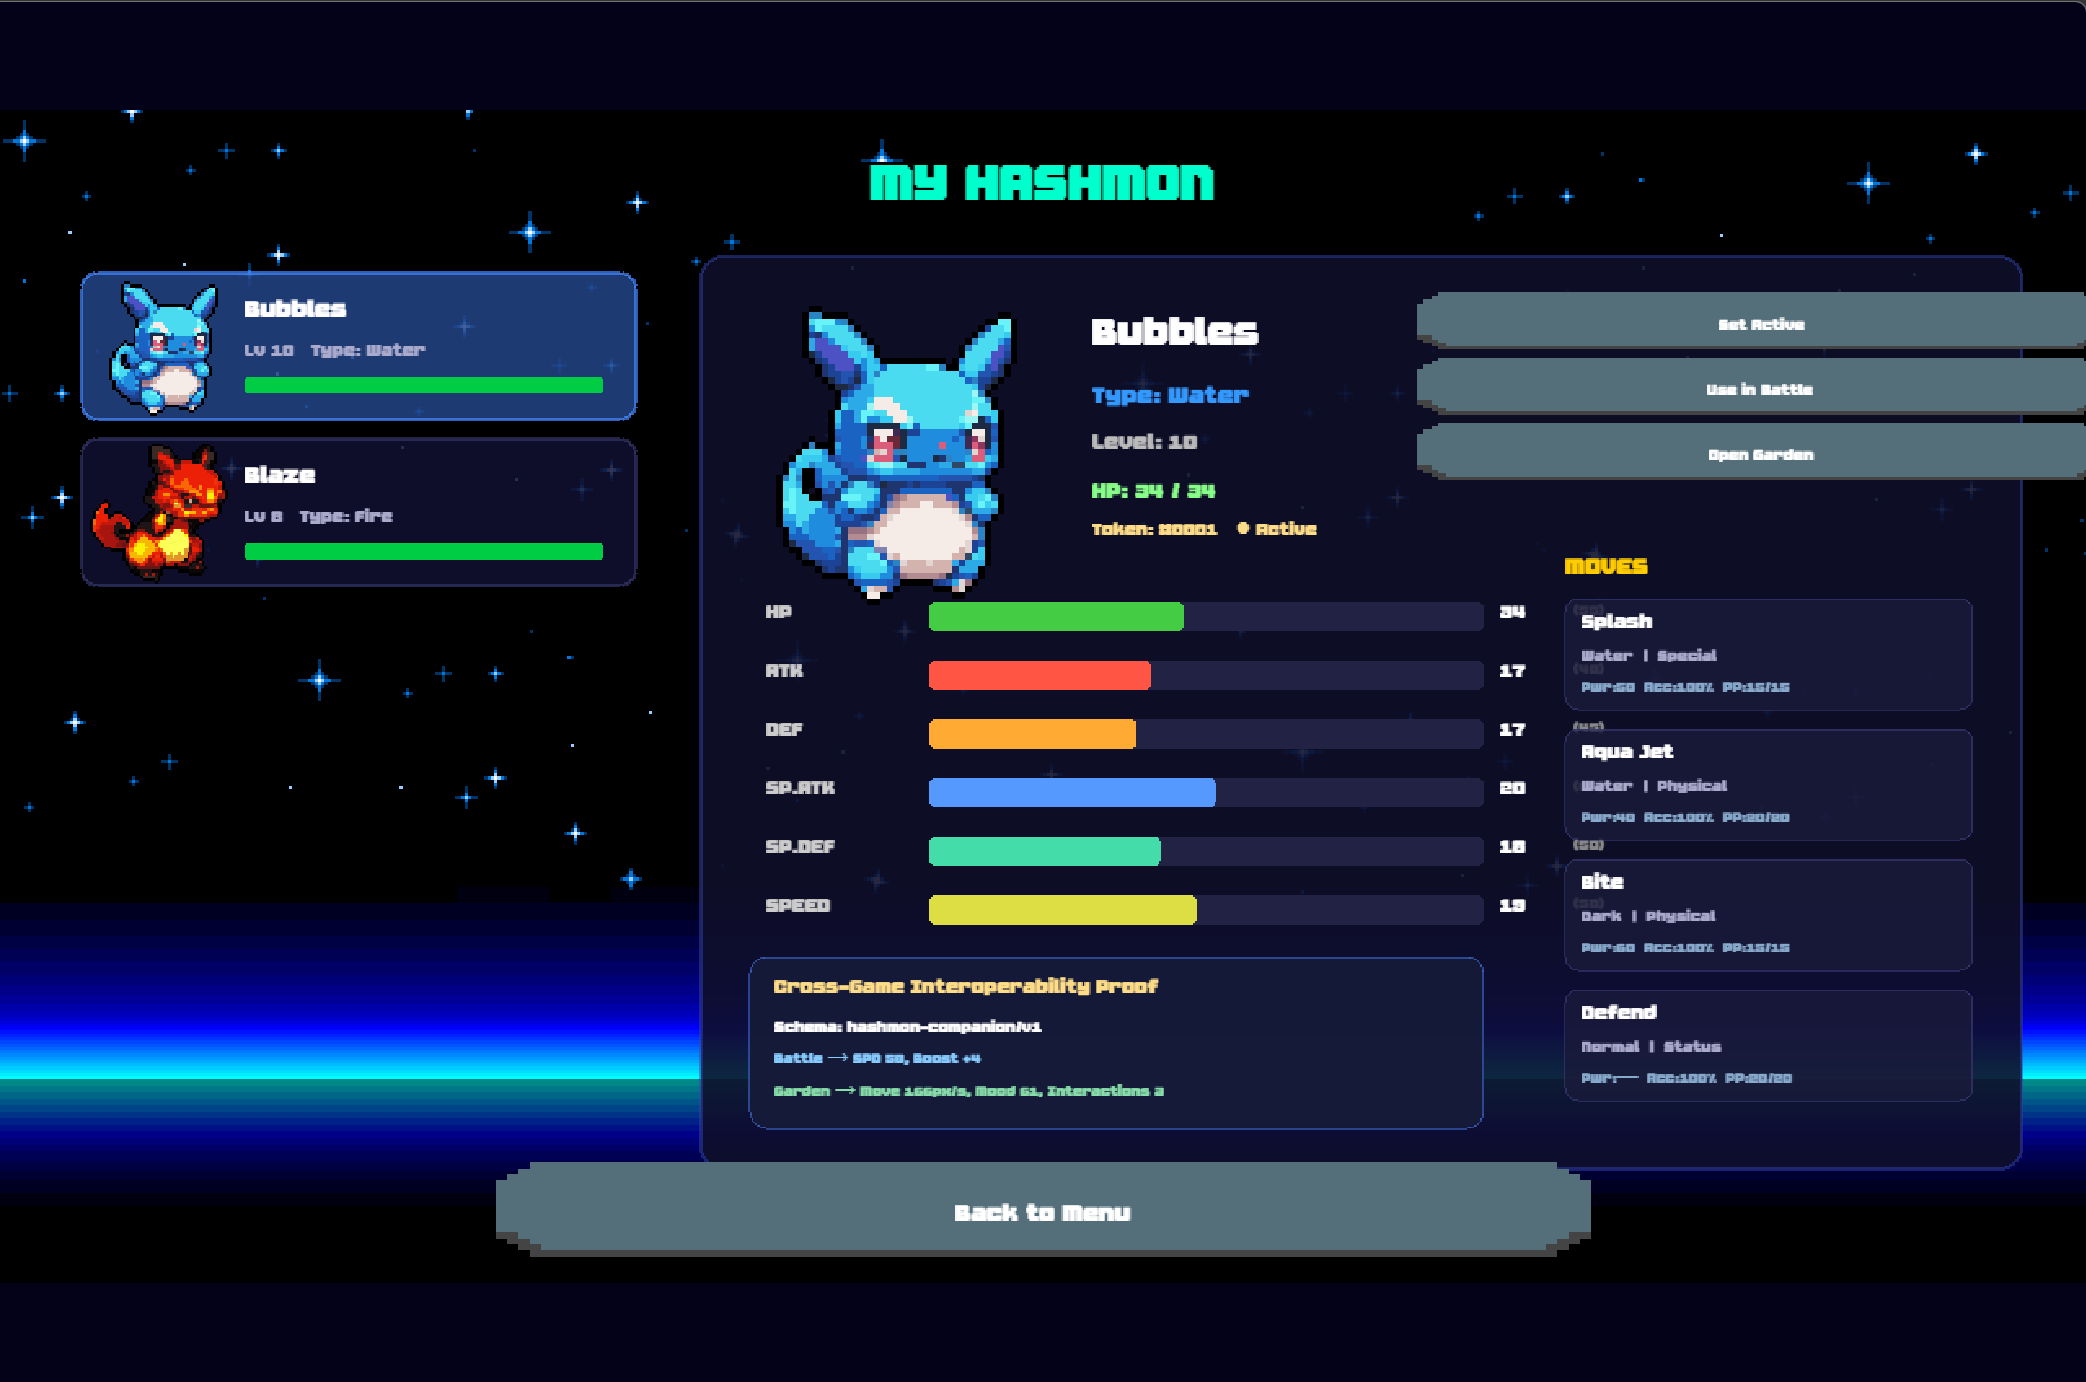
\includegraphics[height=0.22\textheight,keepaspectratio]{MyhashmonScene.png}
    \caption{Detailed My Hashmon management scene.}
  \end{subfigure}
  \hfill
  \begin{subfigure}{0.48\textwidth}
    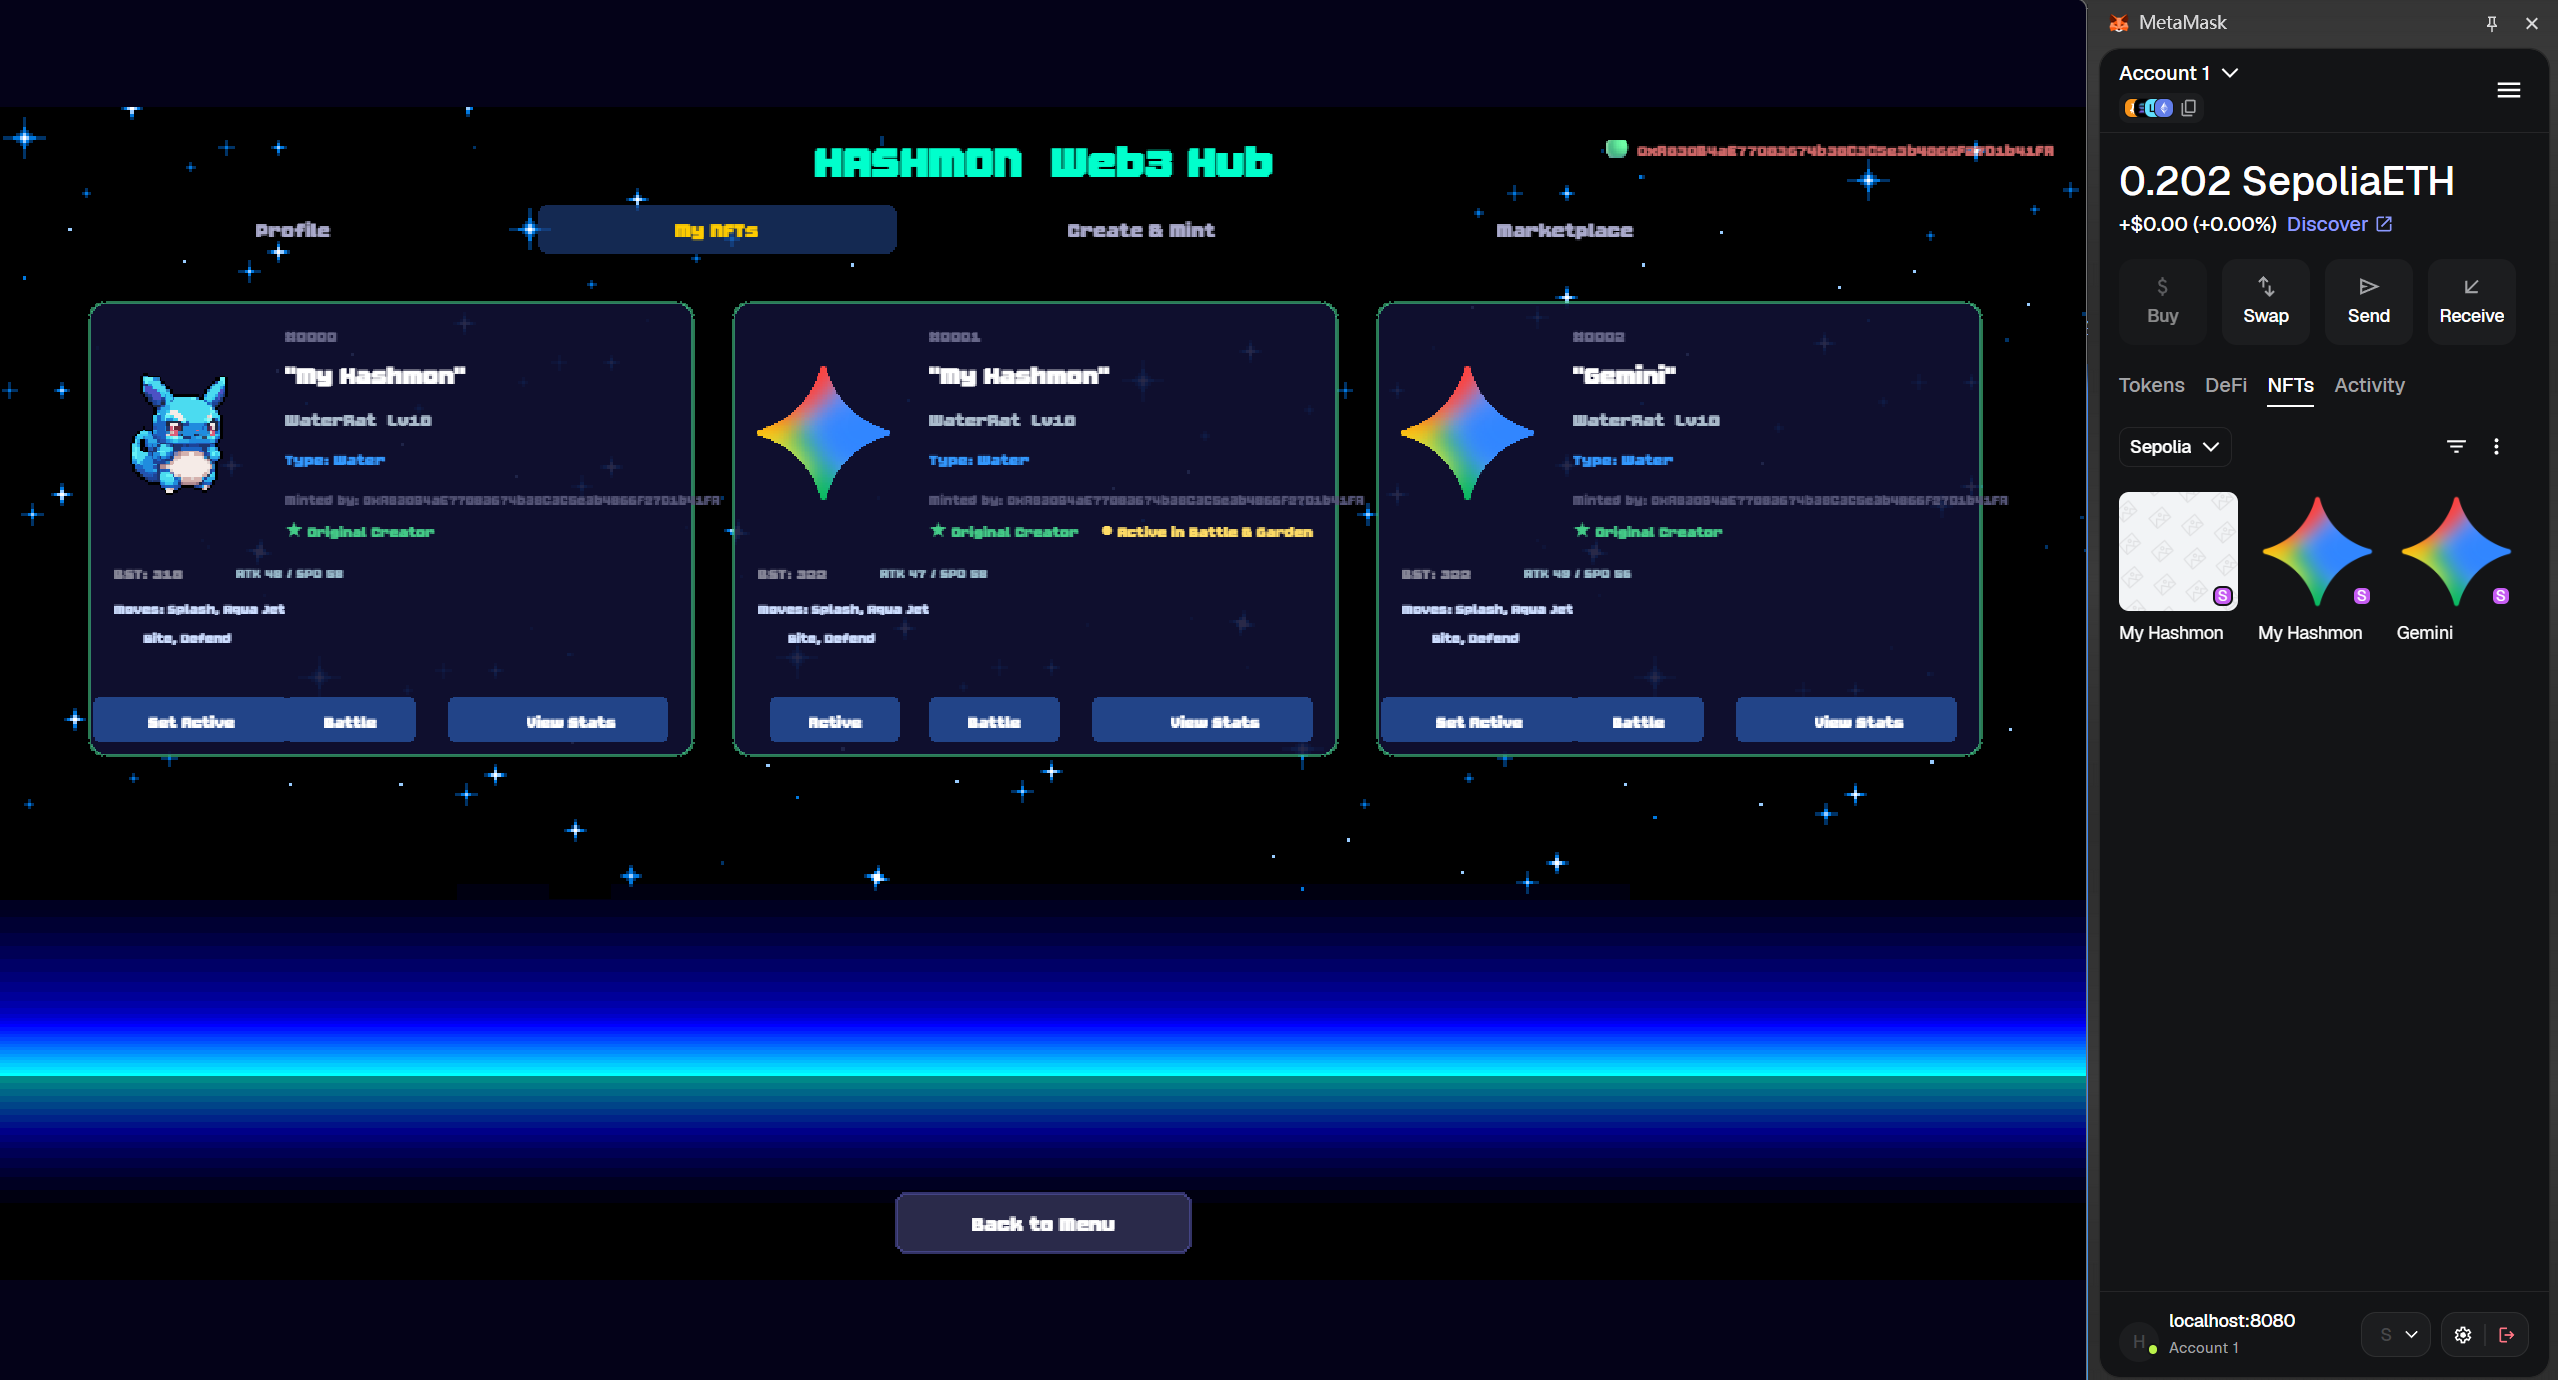
\includegraphics[height=0.22\textheight,keepaspectratio]{AllMintedHashmons.png}
    \caption{Global overview of minted Hashmon assets.}
  \end{subfigure}
  \caption{Wallet-derived ownership and inventory views after NFT minting.}
  \label{fig:ownership-views}
\end{figure*}

These interfaces collectively demonstrate that the NFT is not treated as an isolated token identifier. Instead, the token becomes part of the player-facing companion management loop, making ownership visible, inspectable, and actionable within the game client.

From an engineering standpoint, one of the most important implementation upgrades was the introduction of an \emph{active companion} mechanism. Instead of relying on scene-local demo data, the system allows one user-owned NFT to be selected as the currently active Hashmon. This active asset is then consumed by both the battle and garden modules. Metadata normalization and lightweight state management are handled in the shared player profile and companion protocol code.

A second major engineering decision was the division between on-chain and off-chain information. The NFT contract stores ownership and metadata pointers, which provide persistence and transferability. The IPFS layer stores richer descriptive content such as artwork and structured metadata fields. Meanwhile, the game client interprets this metadata in real time and maintains lightweight gameplay progression during a session. This division was chosen because it balances decentralization with usability: critical identity and ownership stay verifiable on-chain, while richer media and fast-changing interface state remain efficient to manage.

The implementation process also highlighted practical development challenges typical of Web3 frontends. Wallet connection needs to be resilient to browser state and user permission flow; metadata retrieval needs to handle asynchronous loading and inconsistent gateways; and scene synchronization needs to avoid drifting into hardcoded demo data. Solving these issues was not only an engineering task but also part of the research contribution, because the final prototype had to show a believable end-to-end experience rather than isolated technical fragments.

\section{Controlled Interoperability Demonstration}
The central research question of this project is what interoperability should mean in a realistic course-scale system. The answer provided by Hashmon is not universal asset portability across the entire game industry, but a controlled and verifiable proof that the same NFT can preserve identity and selected meaning across two structurally different gameplay environments. We term this \emph{controlled interoperability}: one asset, multiple meaningful contexts.

In the \textbf{Battle Scene}, the active Hashmon is interpreted as a turn-based combat unit. Its battle-related statistics influence health, damage potential, and turn order through the speed attribute. In the \textbf{Garden Scene}, the same Hashmon is interpreted as a roaming pet-like companion whose normalized agility affects movement speed, while interaction counters and happiness values drive mood and behavior feedback.

\begin{figure*}[!tbp]
  \centering
  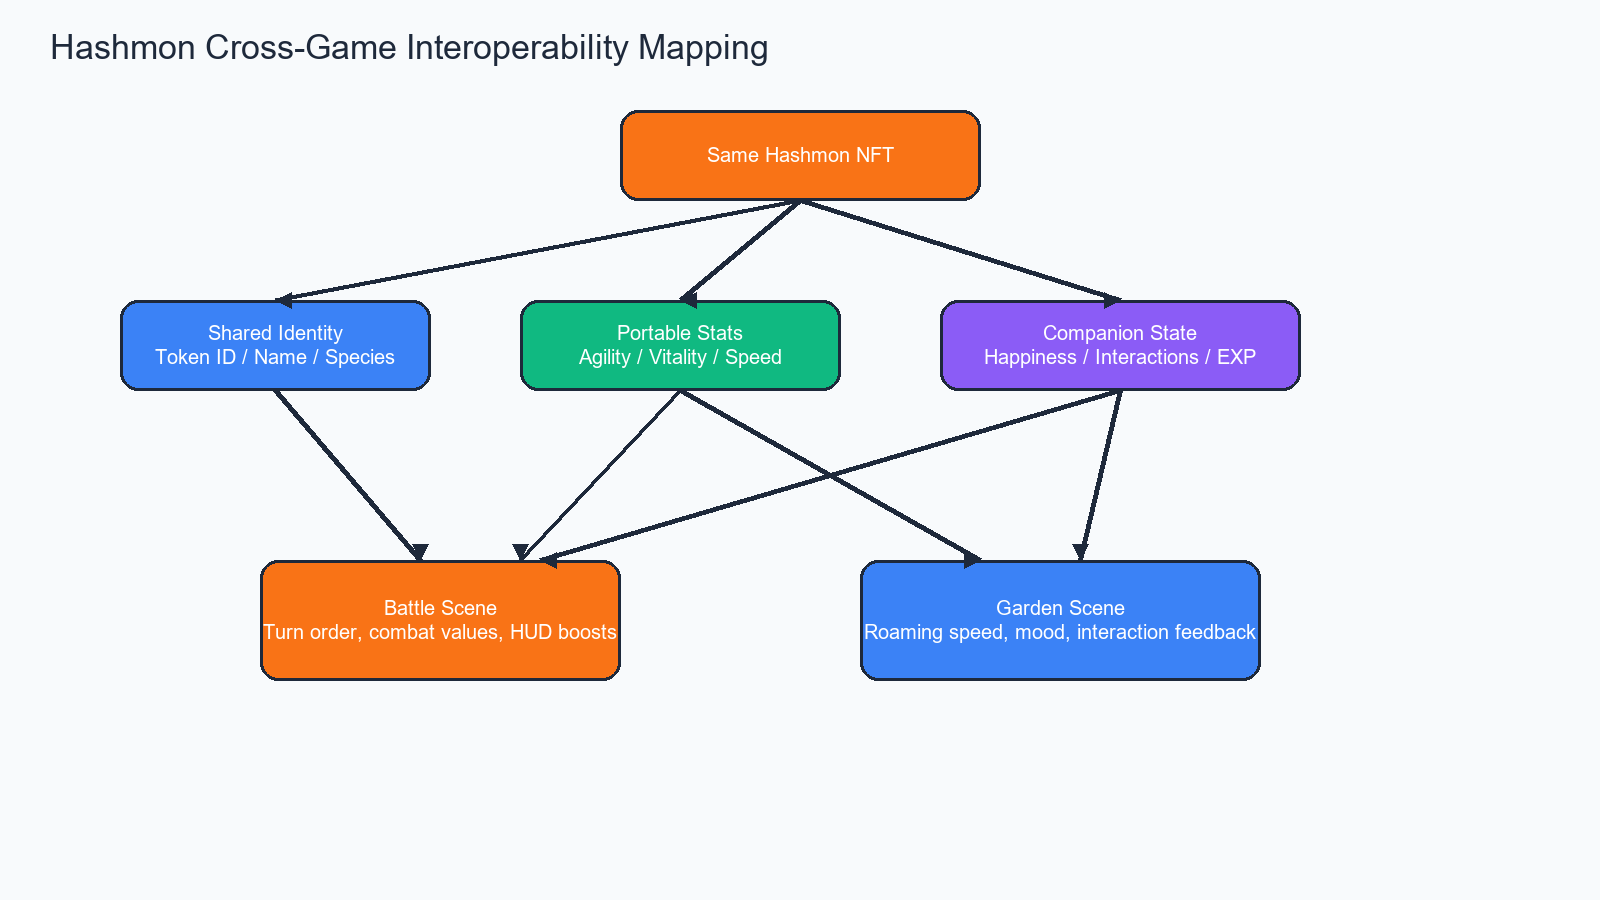
\includegraphics[width=0.92\textwidth]{graphs/hashmon_interoperability_mapping.png}
  \caption{Controlled interoperability mapping for the same NFT companion across different scenes.}
  \label{fig:interop-map}
\end{figure*}

\begin{figure*}[!tbp]
  \centering
  \begin{subfigure}{0.48\textwidth}
    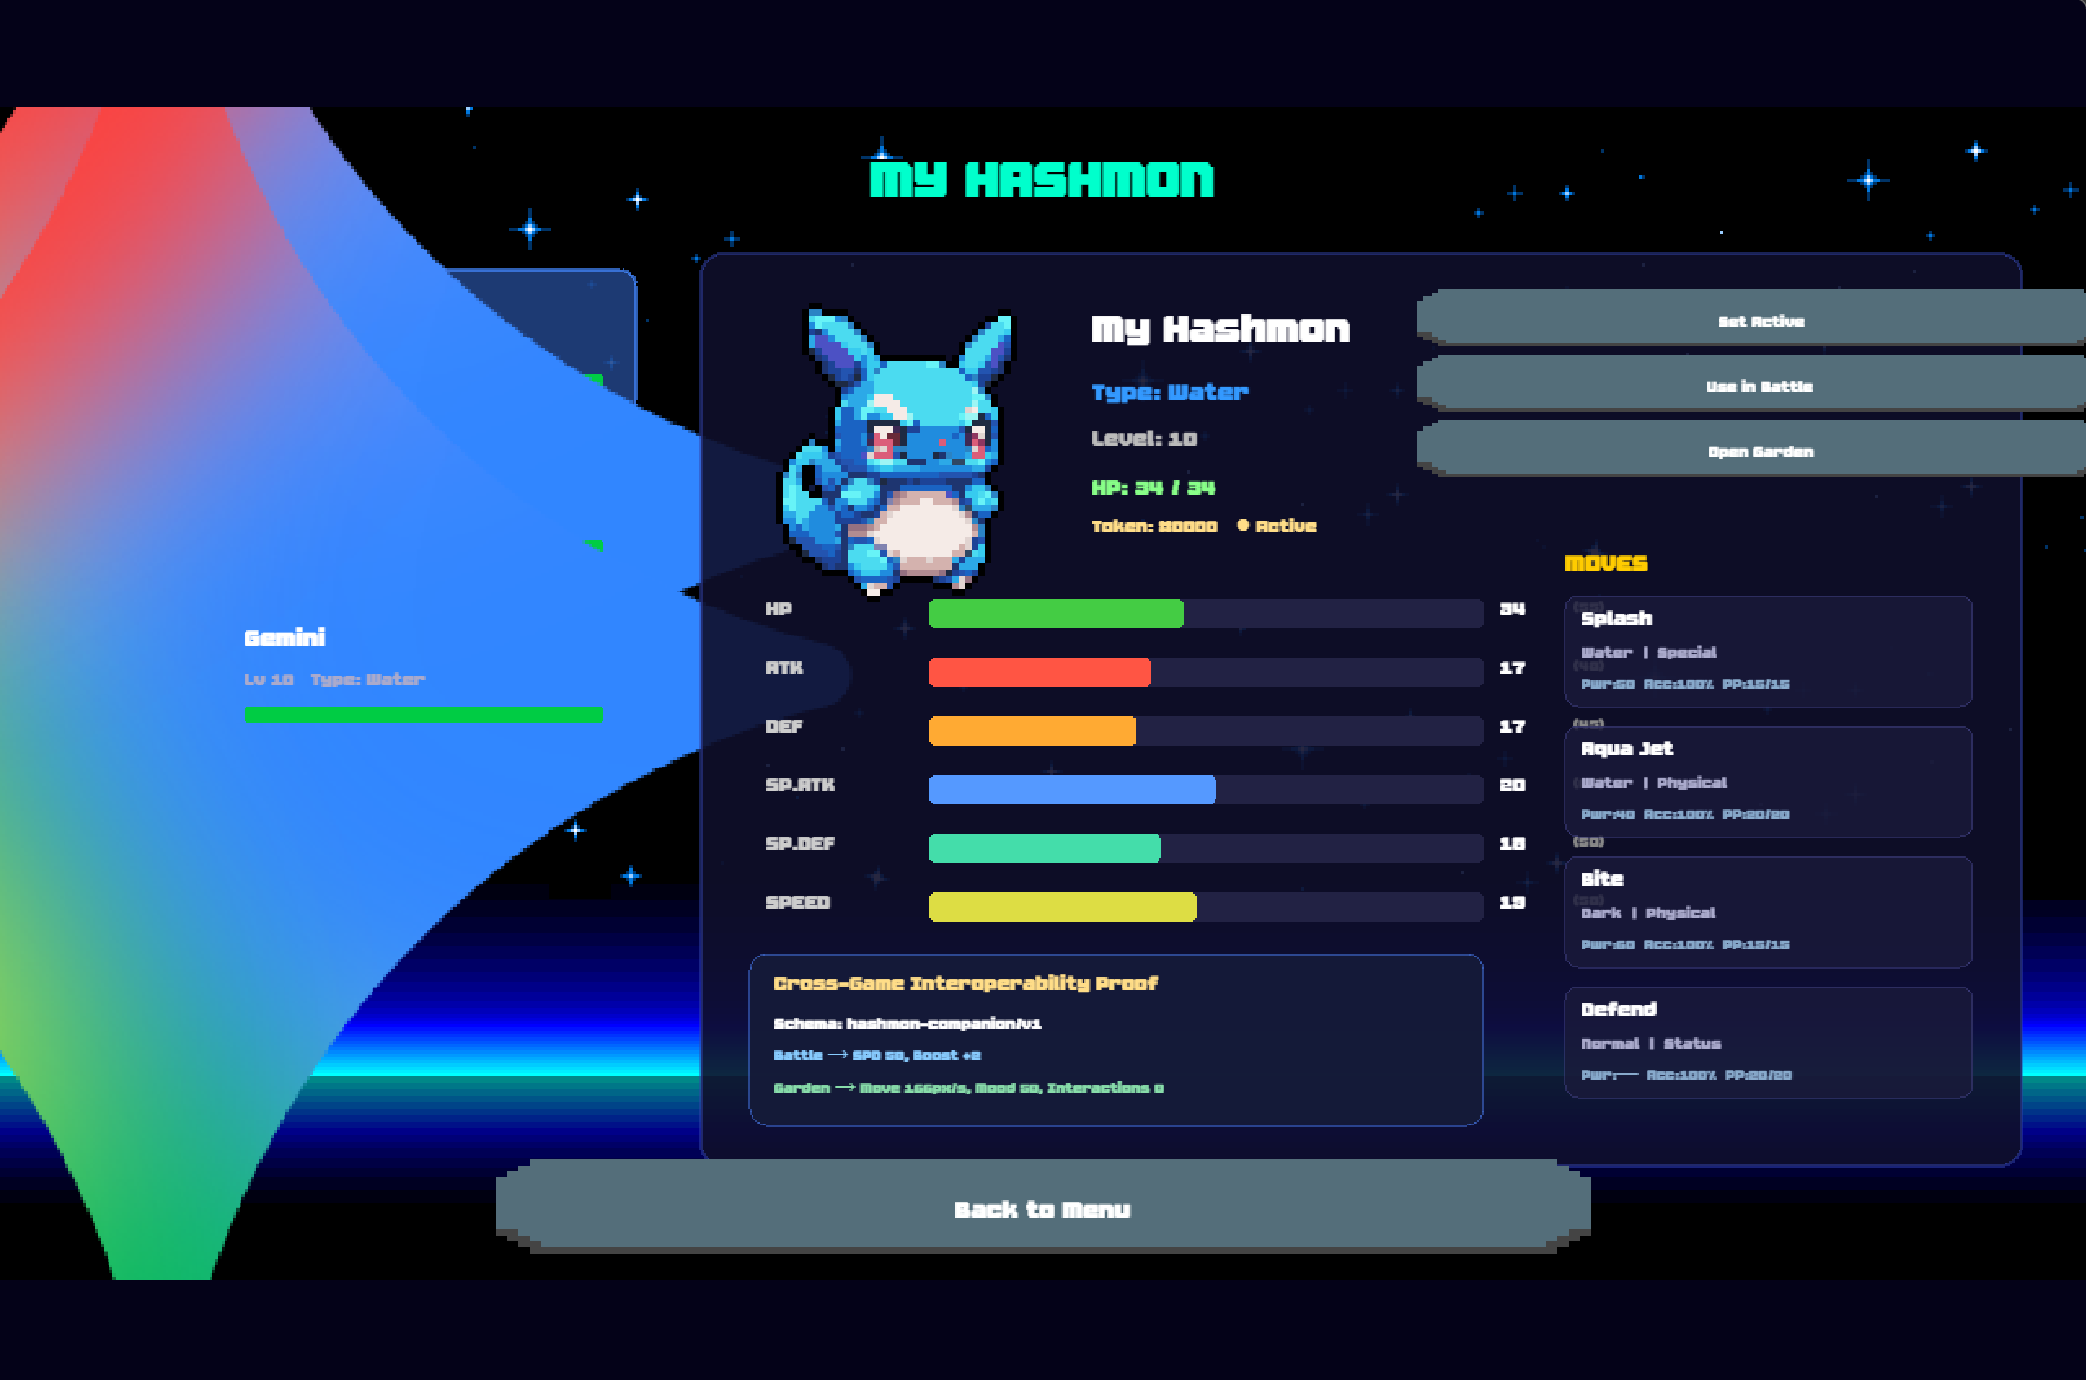
\includegraphics[height=0.22\textheight,keepaspectratio]{StatusWithCrossGameInteroperabilityProof.png}
    \caption{Inventory-based cross-game proof panel.}
  \end{subfigure}
  \hfill
  \begin{subfigure}{0.48\textwidth}
    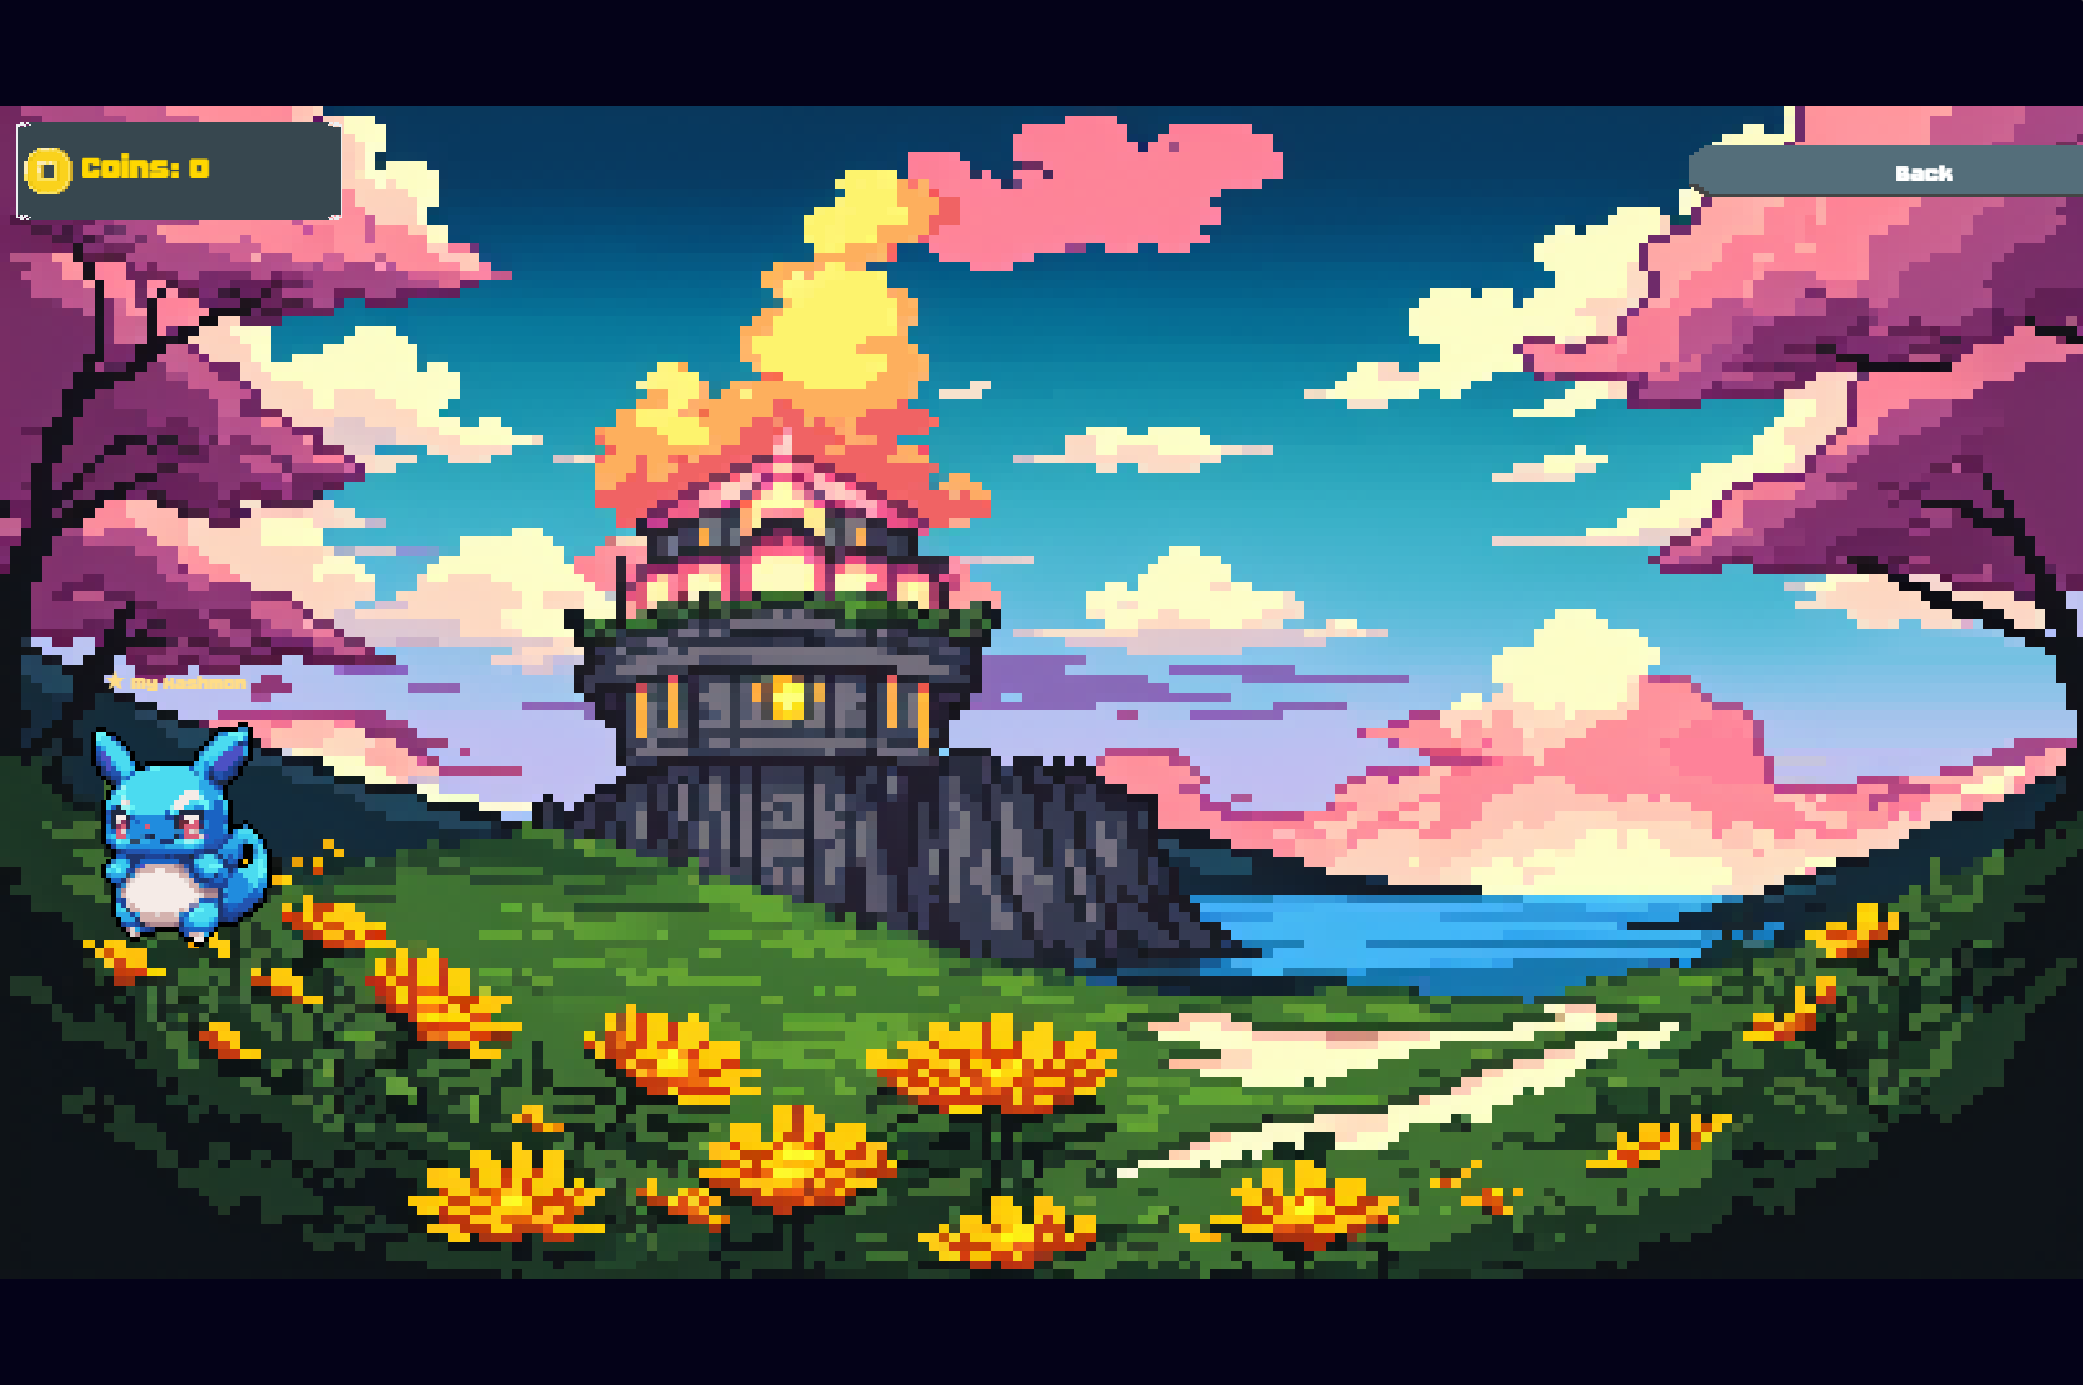
\includegraphics[height=0.22\textheight,keepaspectratio]{GardenScene.png}
    \caption{Garden scene using the active NFT companion.}
  \end{subfigure}

  \vspace{0.6em}

  \begin{subfigure}{0.48\textwidth}
    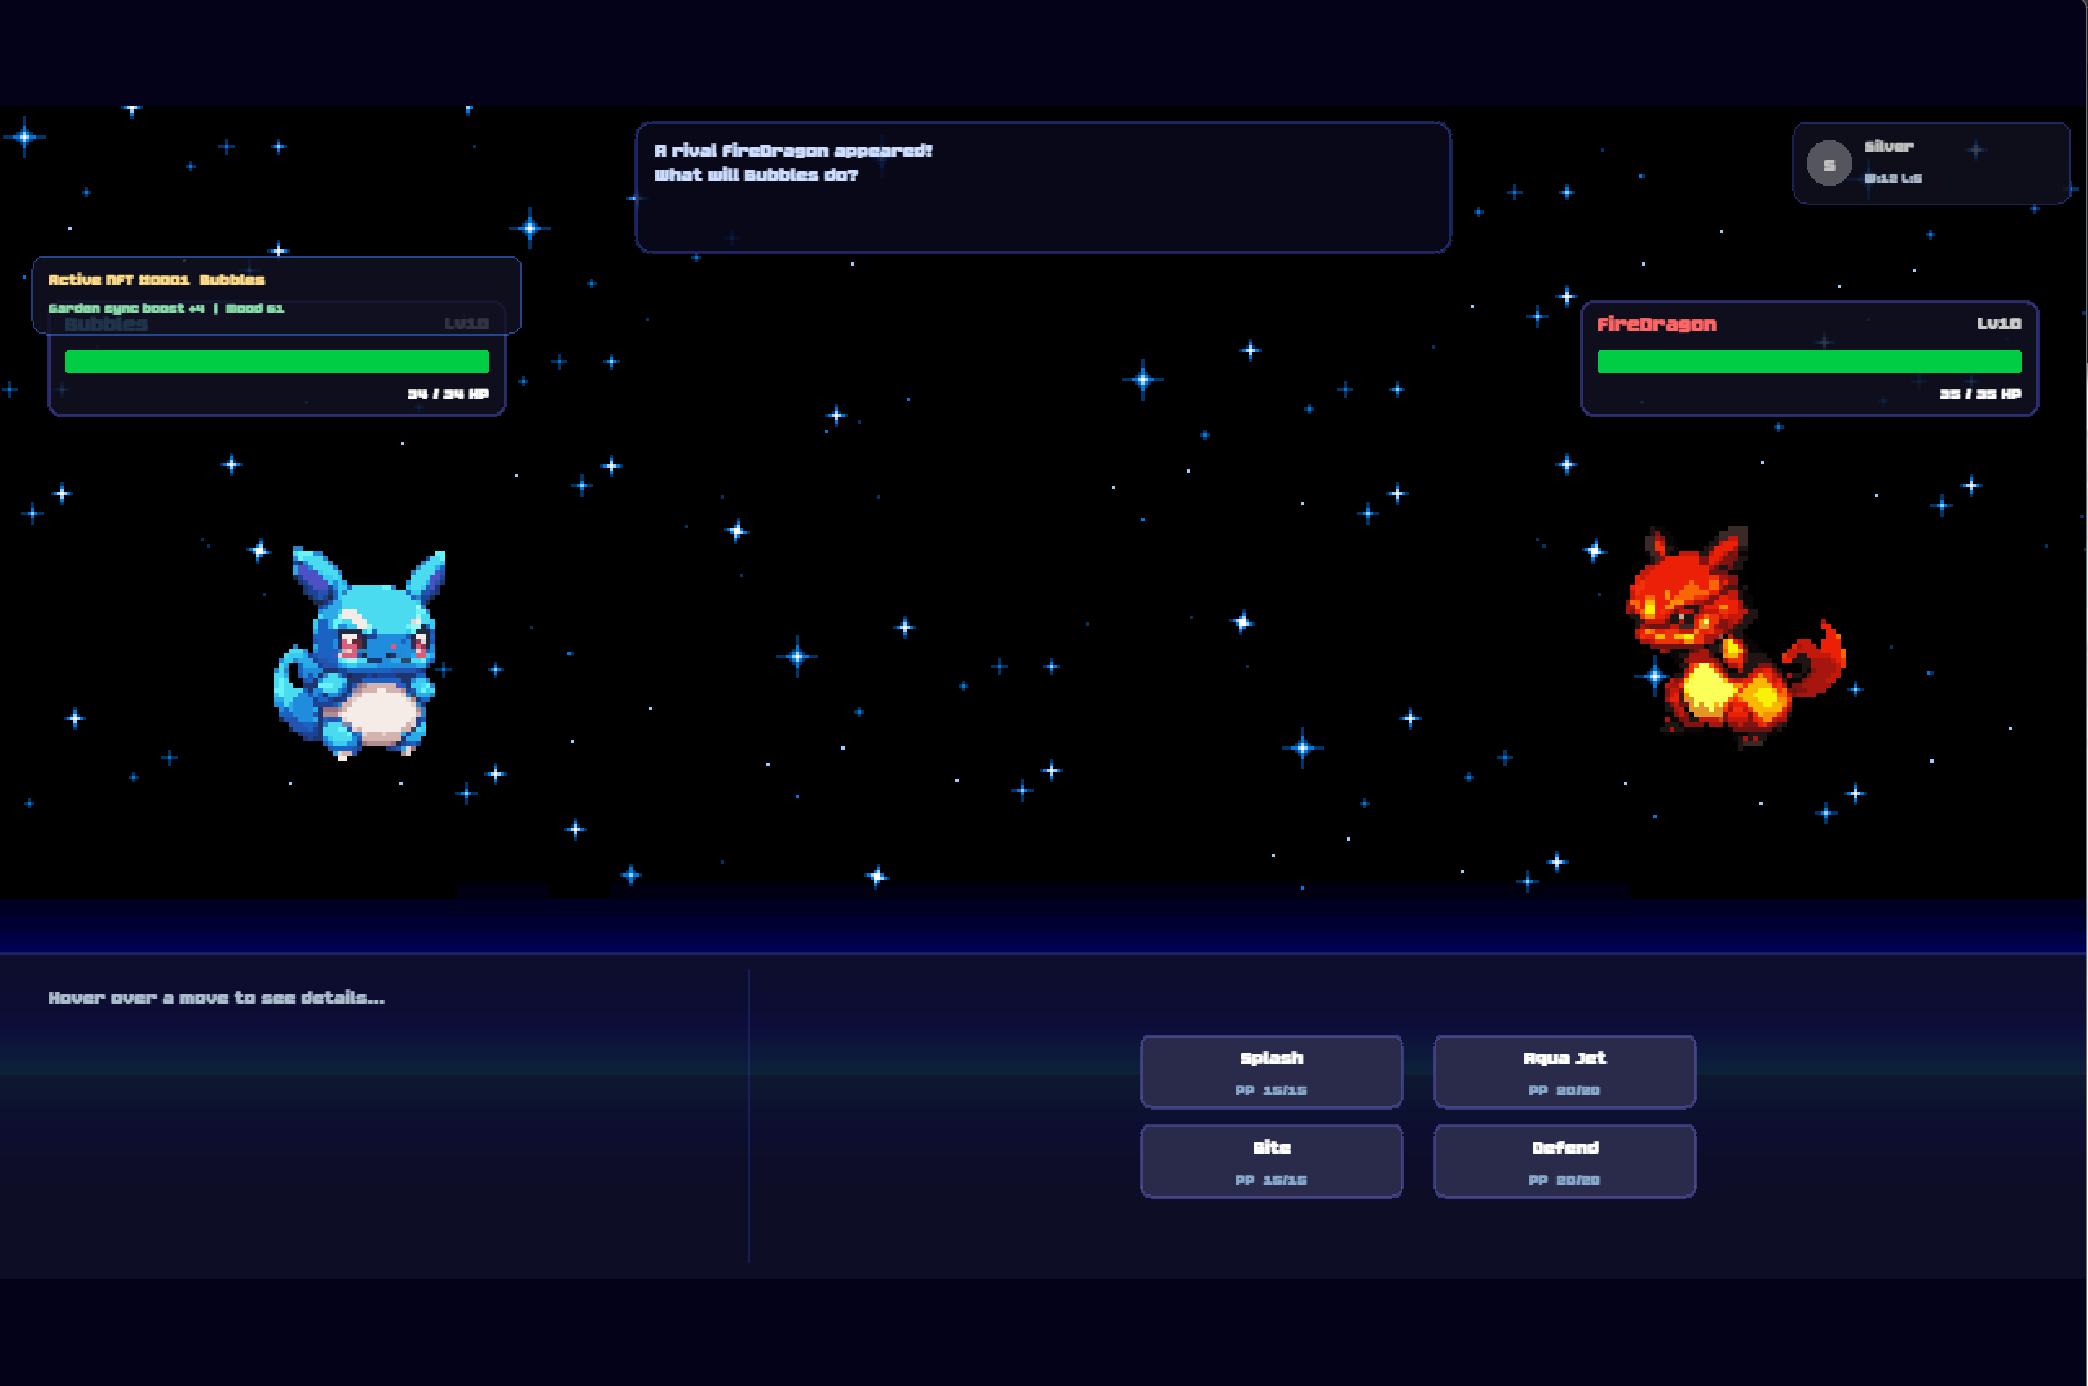
\includegraphics[height=0.23\textheight,keepaspectratio]{BattleScene.png}
    \caption{Battle scene reusing the same NFT-backed Hashmon.}
  \end{subfigure}
  \caption{Visual evidence of cross-scene NFT reuse in the final prototype.}
  \label{fig:interop-proof}
\end{figure*}

This mapping solves a key conceptual issue: the same numeric fields are not blindly reused, but reinterpreted through scene-specific adapters. For example, agility can influence roaming behavior in the garden while speed influences turn order in battle. In addition, interactions performed in the garden increment lightweight companion state such as happiness and experience, which is then surfaced again when the NFT appears in the battle scene. This establishes a basic but concrete form of state carryover.

\section{Prototype Demonstration Scenarios}
To make the prototype easier to evaluate, the final system can be understood through four demonstration scenarios.

\textbf{Scenario 1: Wallet onboarding.} A user launches the game, enters the Web3 hub, and authorizes MetaMask. This creates the bridge between off-chain gameplay and on-chain ownership.

\textbf{Scenario 2: User-generated companion minting.} The player creates a personalized Hashmon, uploads artwork and metadata, and mints the companion as an NFT on Sepolia. This validates the project's user-generated asset pipeline.

\textbf{Scenario 3: Cross-scene reuse.} The player selects an owned NFT as the active companion, then reuses it in both the garden and battle scenes. This demonstrates identity persistence and portable state interpretation.

\textbf{Scenario 4: Marketplace circulation.} The companion can be listed for sale and browsed through the marketplace interface, showing that the NFT is part of a broader asset lifecycle rather than a static trophy.

Together, these scenarios provide a complete narrative for live demo presentation: connect, mint, inspect, reuse, and trade. This sequence also mirrors the practical evaluation criteria applied during development.

\section{Evaluation and Results}
The final system was evaluated primarily as a functional prototype. The main criteria were whether the application could complete the full Web3 loop and whether the interoperability claim could be demonstrated clearly and credibly.

To make this evaluation more systematic, the prototype was tested through repeated end-to-end walkthroughs rather than isolated feature checks. Each walkthrough began from a fresh browser session, proceeded through wallet connection, asset synchronization, and minting, and ended with scene reuse and marketplace interaction. This method was chosen because the main value of the project lies in the continuity of the overall experience, not in any single isolated API call.

The evaluation also focused on consistency. A successful result required that the same companion identity remain recognizable across the inventory, battle, and garden scenes, and that the user could trace a clear line from token ownership to scene participation. This emphasis on continuity is especially important for interoperability claims, since disconnected features do not provide meaningful evidence of portability.

\subsection{Evaluation Dimensions}
Beyond simple feature completeness, the project was evaluated along four dimensions: ownership validity, content persistence, cross-scene reuse, and user-facing clarity. Ownership validity asks whether the minted asset is genuinely tied to the connected wallet. Content persistence asks whether artwork and metadata remain retrievable through the IPFS-backed token URI. Cross-scene reuse asks whether the selected NFT can be meaningfully consumed by more than one gameplay environment. User-facing clarity asks whether the demo is understandable enough for an evaluator to follow without needing access to internal source code.

\begin{table}[t]
  \caption{Functional evaluation of the Hashmon prototype.}
  \label{tab:features}
  \centering
  \begin{tabular}{p{0.40\linewidth}p{0.16\linewidth}p{0.30\linewidth}}
    \toprule
    Feature & Status & Evidence \\
    \midrule
    Local game launch & Yes & Start scene \\
    MetaMask wallet connection & Yes & Web3 hub screenshots \\
    User-customized NFT minting & Yes & Create-and-mint flow \\
    IPFS image and metadata upload & Yes & Mint process \\
    NFT retrieval from wallet & Yes & Inventory view \\
    Marketplace listing and browsing & Yes & Marketplace scene \\
    Cross-scene active companion reuse & Yes & Battle and garden scenes \\
    Interoperability proof panel & Yes & Inventory proof view \\
    \bottomrule
  \end{tabular}
\end{table}

The results confirm that Hashmon successfully supports all five core Web3 interactions end-to-end on the Sepolia testnet. More importantly, the interoperability proof is not limited to showing the same picture twice: it demonstrates identity persistence, asset reuse, scene-specific reinterpretation of shared attributes, and limited state carryover between environments.

\subsection{Quantitative Observations}
To supplement the qualitative walkthrough, several on-chain and network-level metrics were recorded during repeated testing sessions. These measurements cover real blockchain transactions and real IPFS gateway resolution, and are therefore independent of the local development environment.

\begin{table}[t]
  \caption{Quantitative metrics from Sepolia deployment and IPFS gateway testing.}
  \label{tab:quant}
  \centering
  \begin{tabular}{p{0.44\linewidth}p{0.42\linewidth}}
    \toprule
    \textbf{Metric} & \textbf{Observed Value} \\
    \midrule
    Mint transaction cost          & 0.02 SepoliaETH per mint \\
    Mint transactions tested       & 4 (all confirmed) \\
    Mint success rate              & 100\% (4/4) \\
    Token URI resolve success rate & 100\% (10/10 consecutive) \\
    IPFS metadata availability     & All pinned assets retrievable via Pinata gateway \\
    \bottomrule
  \end{tabular}
\end{table}

The consistency of the mint cost across four separate transactions (0.02~SepoliaETH each, spanning April~16--18, 2026) indicates stable contract behavior under the current Sepolia gas conditions. The 100\% token URI resolve rate over ten consecutive refreshes confirms that IPFS-pinned metadata remains reliably accessible through the Pinata gateway, which is important for the prototype's claim that companion identity persists outside the game frontend.

To present these results in perspective, Table~\ref{tab:strengths-challenges} summarizes the verified capabilities alongside the remaining open challenges.

\begin{table}[t]
  \caption{Prototype capabilities versus open challenges.}
  \label{tab:strengths-challenges}
  \centering
  \begin{tabular}{p{0.42\linewidth}p{0.42\linewidth}}
    \toprule
    \textbf{Prototype Demonstrates} & \textbf{Open Challenges} \\
    \midrule
    Wallet-based authentication    & Multi-chain support \\
    On-chain NFT minting (ERC-721) & Deeper gameplay mechanics \\
    IPFS-hosted metadata \& art    & Cross-project standard adoption \\
    Cross-scene companion reuse    & Game balance across contexts \\
    Peer-to-peer marketplace       & UI polish \& user testing \\
    \bottomrule
  \end{tabular}
\end{table}

Crucially, the limitations listed on the right are matters of \emph{engineering scope}, not architectural feasibility. The core design --- layered architecture, companion protocol, pipeline-then-fan-out workflow --- holds and can be extended without fundamental redesign.

For the scope of an undergraduate course project, this constitutes a meaningful and credible proof-of-concept. The prototype does not solve the general problem of cross-studio interoperability, but it validates a concrete architecture that future work can extend.

\subsection{Observed Strengths of the Prototype}
Several strengths became clear during the final integration and demonstration process. First, the prototype provides a rare combination of user-generated content and on-chain ownership within a lightweight browser game. This makes the system immediately understandable to a course evaluator: the user can see what was created, what was minted, and how it is reused. Second, the active-companion mechanism makes the interoperability claim tangible instead of abstract. Third, the marketplace flow demonstrates that the NFT also participates in an economic lifecycle beyond scene rendering.

Another strength is the coherence of the user story. The prototype does not merely expose a set of technical endpoints; it gives the player a narrative sequence in which a companion is born, owned, carried into different contexts, and potentially exchanged. This coherence improves the explanatory power of the project and aligns well with the broader design motivation of preserving attachment to long-lived digital companions.

\section{Discussion}
The most important lesson from this project is that ownership alone is not enough. Simply minting a game creature as an NFT does not automatically make it interoperable. What matters is the protocol layer that defines which parts of the companion's identity and behavior are portable across contexts. In Hashmon, this meant building a lightweight semantic bridge between wallet ownership, metadata, and scene-specific gameplay logic.

A second lesson is that usability matters as much as blockchain functionality. During implementation, features such as clear wallet feedback, visible inventory synchronization, and intuitive scene navigation were essential for making the prototype understandable to evaluators. In a course project, technical correctness and presentation clarity reinforce each other.

Finally, the project suggests that Web3 can be most compelling in games when it supports long-term emotional attachment rather than purely speculative asset trading. The idea of carrying a familiar companion into future experiences is a stronger design motivation than tokenization alone, and it points toward more player-centered Web3 game systems.

A related reflection concerns scope management. Early in the project, it was tempting to describe the system as a broad multi-game platform. In practice, a narrower claim produced a stronger result. By concentrating on a controlled proof of interoperability rather than a vague promise of universal compatibility, the project became easier to finish, easier to demonstrate, and more persuasive as a technical artifact. This lesson is relevant to many student projects in emerging technology domains: precision of scope often improves both credibility and implementation quality.

\section{Limitations and Future Work}
The project has several acknowledged limitations. First, the current implementation only demonstrates interoperability across two controlled scenes within one prototype. A truly open ecosystem would require broader protocol standardization and adoption by multiple developers. Second, most portable state is still managed at the application layer rather than through full token-bound accounts.

\subsection{Threats to Validity}
As with many prototype-driven studies, several threats to validity should be acknowledged. The evaluation is primarily qualitative and scenario-based rather than based on a large-scale user study. This means that while the system demonstrates feasibility, it does not yet measure broader user acceptance, long-term engagement, or the economic behavior of a larger player community. In addition, because the prototype is built on a controlled Sepolia testnet environment, its operational reliability may differ from a production deployment on a more heavily used network.

Another limitation is the bounded meaning of the companion protocol itself. The protocol currently captures only a compact set of fields that are sufficient for the battle and garden scenes. More diverse future games might require richer semantics for equipment, social relationships, progression trees, or AI-driven behaviors. Therefore, the current system should be understood as a minimal viable interoperability layer rather than a final universal standard.

\subsection{Future Directions}
Four concrete directions can extend the current prototype into a more complete ecosystem.

\textbf{Direction 1: Multi-chain support.} Extending to Layer~2 networks such as Polygon or Arbitrum would reduce transaction costs and improve responsiveness, making the system viable for a wider player base.

\textbf{Direction 2: Richer gameplay mechanics.} Integrating evolution, breeding, equipment systems, and deeper battle mechanics would make the companion protocol more expressive and the cross-scene reuse more meaningful.

\textbf{Direction 3: Open companion metadata standard.} Proposing the companion protocol as an Ethereum Improvement Proposal (EIP) draft would allow other developers to build compatible mini-games that can read the same NFT companion and interpret its state according to their own mechanics. This would move the project one step closer to a genuine multi-experience companion ecosystem.

\textbf{Direction 4: Community governance.} Transitioning marketplace governance to a DAO structure would enable community ownership of the protocol's evolution, moving beyond a single-developer prototype toward a player-governed ecosystem.

Additional improvements include ERC-6551~\cite{erc6551} token-bound accounts so that each Hashmon may directly hold items and persistent progression on-chain, stronger backend security for IPFS credential handling, and support for richer avatar or 3D asset formats that more closely match the original long-term platform vision.

\section{Conclusion}
Hashmon demonstrates that a player-created companion can become a persistent digital asset with verifiable ownership and controlled reuse across multiple gameplay contexts. By combining ERC-721 ownership, IPFS-based metadata, a four-layer browser-based architecture, and a lightweight companion protocol, the system proves that cross-game interoperability can be made concrete, testable, and demonstrable in a controlled environment.

The core insight of this project is that ownership alone does not produce interoperability. What makes the companion \emph{meaningful} across scenes is the protocol layer that defines which parts of its identity and behaviour are portable, and the scene-specific adapters that reinterpret those shared attributes according to each gameplay context. This principle --- controlled interoperability through a semantic bridge --- provides a solid technical foundation and a credible research direction for future Web3-native game ecosystems centered on persistent, player-owned companions.

\section*{Contribution Statement}
The frontend implementation, Web3 integration, smart contract debugging, IPFS pipeline, interoperability design, report drafting, and presentation preparation were completed primarily by Baohua Fang (ID: 123090108). The other student in the group, Qijia Bai (ID: 122090001), has done nothing at all. The final workload distribution of the project was significantly uneven.

\bibliographystyle{ACM-Reference-Format}
\bibliography{references}

\end{document}
